\section{Glatte Mannigfaltigkeiten und Tangentialbündel}
\label{Mfn}
\subsection{Definitionen einer (Unter)Mannigfaltigkeit}
\label{subsec:Umfn}
\begin{definition}{Untermannigfaltigkeit}{umfn}
Eine Teilmenge $M \subseteq \R^n$ ist eine $k$\textbf{-dim. Untermannigfaltigkeit (UMF) des }$\R^k$, falls jeder Punkt $p \in M$ eine offene Umgebung $U \subseteq \R^n$ besitzt, sodass ein Diffeomorphismus
\begin{equation}
h: U \to V 
\end{equation}
mit $V \subseteq \R^n$ offen existiert, für den $h(U \cap M) = V \cap \R^k \times \{0\}^{n-k}$ gilt.
\end{definition}
\begin{bemerkungen}{Andere Definitionen von UMFn}\\
Äquivalent dazu sind die folgenden Formulierungen:
\begin{enumerate}
\item Zu jedem Punkt $x \in M$ existiert eine offene Umgebung $U \subseteq \R^n$ und eine glatte Abbildung 
\begin{equation}
\phi: U \to \R^{n-k},
\end{equation}
sodass gilt:
\begin{itemize}
\item $\forall p \in U \cap M$ hat die Ableitung $d\phi_p: \R^n \mapsto \R^{n-k}$ vollen Rang $n-k$.
\item Es gilt $U \cap M = \phi^{-1}(0)$.
\end{itemize}
\item Zu jedem Punkt $x \in M$ existiert eine offene Umgebung $U \subseteq \R^n$ und eine offene Teilmenge $V^* \subseteq \R^k$ sowie eine glatte Abbildung 
\begin{equation}
\phi: V^* \to \R^n,
\end{equation}
sodass gilt:
\begin{itemize}
\item $\forall y \in V^*$ hat die Ableitung $d\phi_y: \R^k \mapsto \R^n$ vollen Rang $k$.
\item $\phi$ bildet $V^*$ homöomorph auf $U \cap M$ ab.
\end{itemize}
\end{enumerate}
\end{bemerkungen} 
\begin{beweis}
Übung (A1)
\end{beweis}
\begin{figure}[h!]
\label{fig:umfn}
\centering
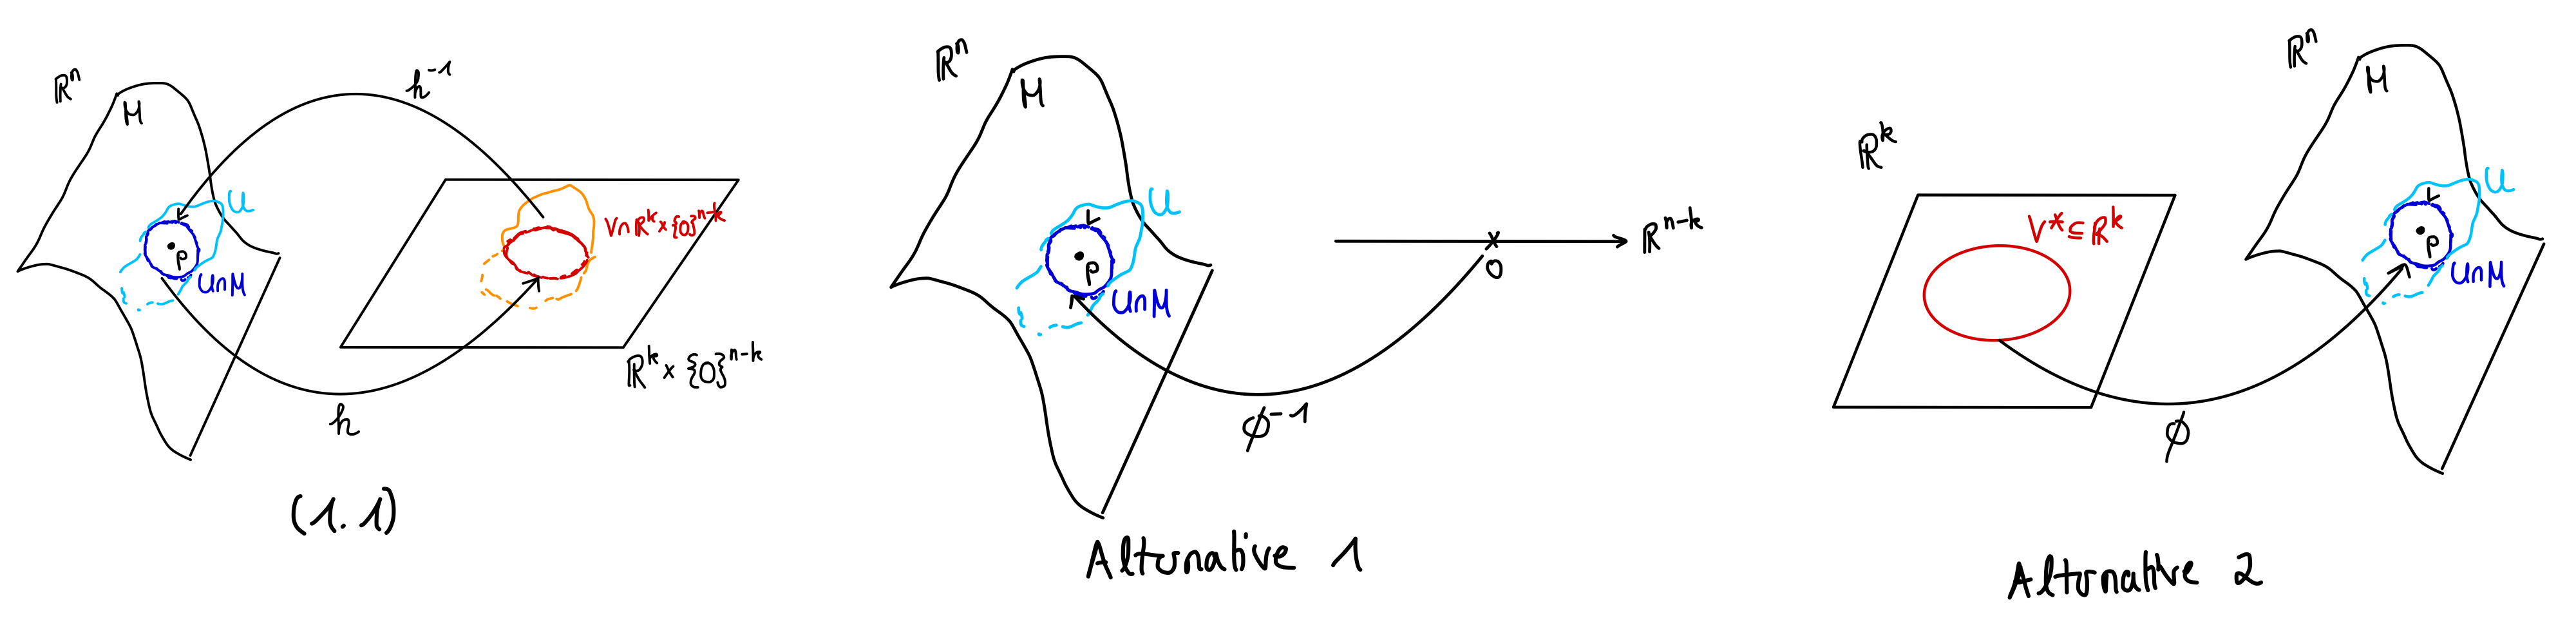
\includegraphics[width=0.9\linewidth]{Bilder/umf_def.png}
\caption{Die verschiedenen Definitionen von UMF.}
\end{figure}
Wir betrachten zwei Beispiele für Untermannigfaltigkeiten:
\begin{beispiele}{verschiedene Untermannigfaltigkeiten}
\begin{enumerate}
\item Betrachte die $k$-dim. Sphäre $\mathbb{S}^k := \{x \in \R^{k+1} | ||x||^2 = \sum_j x_j^2 = 1 \} \subseteq \R^{k+1}$. Wir definieren
\begin{align}
\psi: \R^{k+1} &\to \R \\
x &\mapsto 1-||x||^2 = 1 - \ip{x, x}.
\end{align}
Dann gilt für die Ableitung an $v \in \sph^k$ in Richtung $x$: $\diff \psi_x (v) = -2 \ip{x, v} \neq 0 \forall x \in \mathbb{S}^k$. Also hat das Differential vollen Rang und ist somit surjektiv. Um die Bedingung aus der Definition nachzuprüfen, geht man wie folgt vor: Sei $x \in \sph^k$. O.B.d.A. gilt $x_1 > 0$. Wir wählen $U := \{ x \in \R^{k+1} | x_1 > 0 \}$ und betrachten eine Funktion $h: U \to \R^k, (x_1, \dots, x_{k+1}) \mapsto (x_1 - \sqrt{1-\Sum{j, 2, k+1} x_j^2}, x_2, \dots, x_{k+1})$. Es gilt $\sum_j x_j^2 =1$, also $x_1^2 = 1-\Sum{j,2,k+1} x_j^2$. 
\item Sei $W \subseteq \R^k$ offen und $f: W \to \R^{n-k}$ eine glatte Abbildung, dann ist der \textbf{Graph von} $f$,
\begin{equation}
\graph f:= \{ (x, f(x) \in W \times \R^{n-k} \} \sub \R^k \times \R^{n-k},
\end{equation}
eine UMF der Dimension $k$ in $\R^n$.
Als Umgebung wählen wir $W \times \R^{n-k} \sub \R^n$ und als Diffeomorphismus $h: U \to \R^k \times \R^{n-k}, (x, y) \mapsto (x, y-f(x))$ respektive $\psi(x,y)=y-f(x)$.
\end{enumerate}
\begin{figure}[H]
\label{fig:graph}
\centering
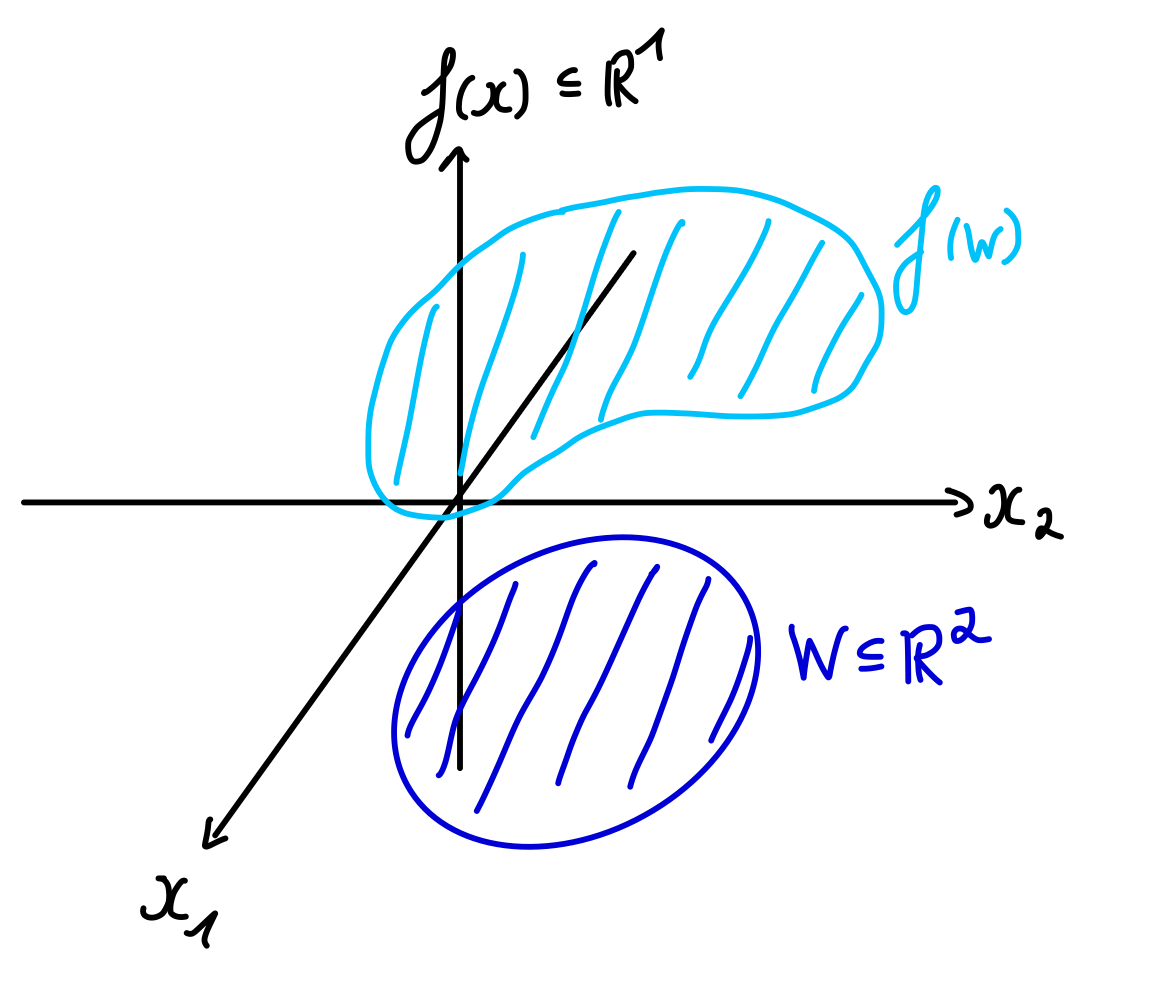
\includegraphics[width=0.2\linewidth]{Bilder/graph.png}
\caption{Der Graph einer Abbildung $f$.}
\end{figure}
\end{beispiele}
\begin{lemma}{Kartenlemma}{kartenlemma}
Sei $M \sub \R^n$ eine $k$-dim. UMF und $p \in M$.\\
Dann existiert eine Umgebung $U \sub \R^n$ von $p$ und eine offene Menge $W \sub \R^k$ sowie eine glatte Abbildung $\phi: W \to U$ mit folgenden Eigenschaften:
\begin{itemize}
\item $\forall y \in W$ hat $\diff \phi_y: \R^k \to \R^k$ maximalen Rang $k$.
\item $\phi$ ist injektiv mit $\phi(W) = U \cap M$.
\end{itemize}
\end{lemma}
\begin{beweis}
Ist $h: U \to V$ ein lokaler Diffeomorphismus wie in \ref{umfn}, können wir $W := \R^k \times \{ 0 \}^{n-k}$ und $\phi: h^{-1}|_W : W \to U \cap M$ betrachten.
\end{beweis}
Es gilt sogar, dass $\phi: W \to U \cap M$ ein Homöomorphismus ist.\\
\begin{theorem}{\textit{Umkehrsatz im} $\R^n$}{kleinerumkehrsatz}
Seien $U,V \sub \R^n$ offen, $p \in U$ und $F: U \to V$ glatt. Ist $F_{\ast,p}$ \textcolor{red}{invertierbar in} $p$, so existieren zusammenhängende Umgebungen $U_0 \sub U$ von $p$ und $V_0 \sub V$ von $F(p)$, sodass
\begin{equation}
F|_{U_0}: U_0 \to V_0
\end{equation} 
ein \textcolor{red}{Diffeomorphismus} ist.
\end{theorem}
\begin{theorem}{\textit{Satz von der impliziten Funktion}}{satzvonderimplizitenfunktion}
Sei $U \sub \R^n \times \R^n$ offen und seien $(x,y) = (x_1, \dots, x_n, y_1, \dots y_n)$ Standardkoordinaten auf $U$. Sei weiterhin $\Phi: U \to \R^k$ eine glatte Funktion, $(a,b) \in U$ und $c=\Phi(a,b)$. Wenn die Matrix
\begin{equation}
\left\{ \frac{\partial \Phi_i}{\partial y_j}(a,b)\right\}
\end{equation}
\textcolor{red}{nicht-singulär} ist, existieren offene Umgebungen $V_0 \sub \R^n$ von $a$, $W_0 \sub \R^k$ von $b$ und eine glatte Funktion $F: V_0 \to W_0$, sodass $\Phi^{-1}(x) \cap (V_0 \times W_0)$ der Graph von $F$ ist, also $\Phi(x,y)=c$ für $(x,y) \in V_0 \times W_0$ genau dann, wenn $y=F(x)$.
\end{theorem}
\begin{definition}{Topologische Mannigfaltigkeit}{topmfn}
Eine \textbf{topologische Mannigfaltigkeit (MFK) der Dimension} $k$ ist ein topologischer Raum $M$ mit folgenden Eigenschaften:
\begin{itemize}
\item $\forall p \in M$ existiert eine offene Umgebung $U$, die homöomorph zu einer offenen Menge $V \sub \R^k$ ist.
\item $M$ ist hausdorffsch.
\item $M$ besitzt eine abzählbare Basis.
\end{itemize}
\end{definition}
\begin{definition}{Hausdorffeigenschaft}{hausdorff}
Ein top. Raum $(X, \Ts)$ heißt \textbf{hausdorffsch}, wenn für alle $x,y \in X, x \neq y$ disjunkte offene Umgebungen $U \in \Ts$ von $x$ und $V \in \Ts$ von $y$ existieren.
\end{definition}
Die wichtigsten Beispiele von Hausdorffräumen sind metrische Räume (dort erfüllt der offene Ball die gewüschten Eigenschaften).
\begin{bemerkung}
Die Forderung der Hausdorffeigenschaft in \ref{topmfn} ist motiviert durch Beispiele folgender Art:\\
Sei $Y := \R \times \{0\} \sqcup \R \times \{1\}$. Wir betrachten die Äquivalenzrelation
\begin{equation}
(t, 0) \sim (s, 1) \iff t=s < 0.
\end{equation} 
Auf $X$ definieren wir eine Topologie: Wie haben Einbettungen
\begin{align}
\iota_0: \R \to X, \ &t \mapsto (t, 0) \\
\iota_1: \R \to X, \ &t \mapsto (t, 1)
\end{align}
und definieren $U \sub X$ als offen genau dann, wenn $\iota_0^{-1} (U)$ offen in $\R$ ist.
\end{bemerkung}
\begin{warning}
Der letzte Teil auf der Tafel wurde nicht mehr hochgeschoben, eine Ergänzung wäre nett.
\end{warning}
\begin{definition}{Basis}{topbasis}
Sei $(X, \Ts)$ ein top. Raum. Eine \textbf{Basis} der Topologie $\Ts$ ist eine Teilmenge $\beta \sub \Ts$ mit der Eigenschaft, dass sich alle offenen $U \in \Ts$ schreiben lassen als Vereinigung $U = \bigcup_{i \in I} B_i$ von $B_i \in \beta$.
\end{definition}
Wir sehen uns ein paar Beispiele an:
\begin{beispiele}{(abzählbare) Basen}
\begin{enumerate}
\item Sei $(X, d)$ ein metrischer Raum. Dann bilden die offenen Bälle eine Basis der Topologie.
\item Der $\R^n$ besitzt eine \textit{abzählbare} Basis. Dazu betrachtet man beispielsweise nur Bälle $\Bs_r(x)$ mit $r, x \in \Q$. Jeder Teilraum erbt diese Eigenschaft.
\end{enumerate}
\end{beispiele}
\begin{definition}{Parakompaktheit}{parakomp}
Ein top. Raum $X$ heißt \textbf{parakompakt}, wenn jede offene Überdeckung von $X$ eine lokal endliche \textit{Verfeinerung} aufweist.\\
Genauer: Ist $\{U_\alpha\}_{\alpha \in A}$ eine beliebige offene Überdeckung von $X$, so existiert eine offene Überdeckung $\{V_\beta \}_{\beta \in B}$ mit zwei Eigenschaften:
\begin{itemize}
\item $\forall \beta \in B \exists \alpha \in A: V_\beta \sub U_\alpha$
\item $\forall x \in X$ existiert ein offenes $U \sub X$ , sodass $\{ \beta \in B | V_\beta \cup U \neq \emptyset \}$ endlich ist.
\end{itemize}
\begin{figure}[H]
\label{fig:parakomp}
\centering
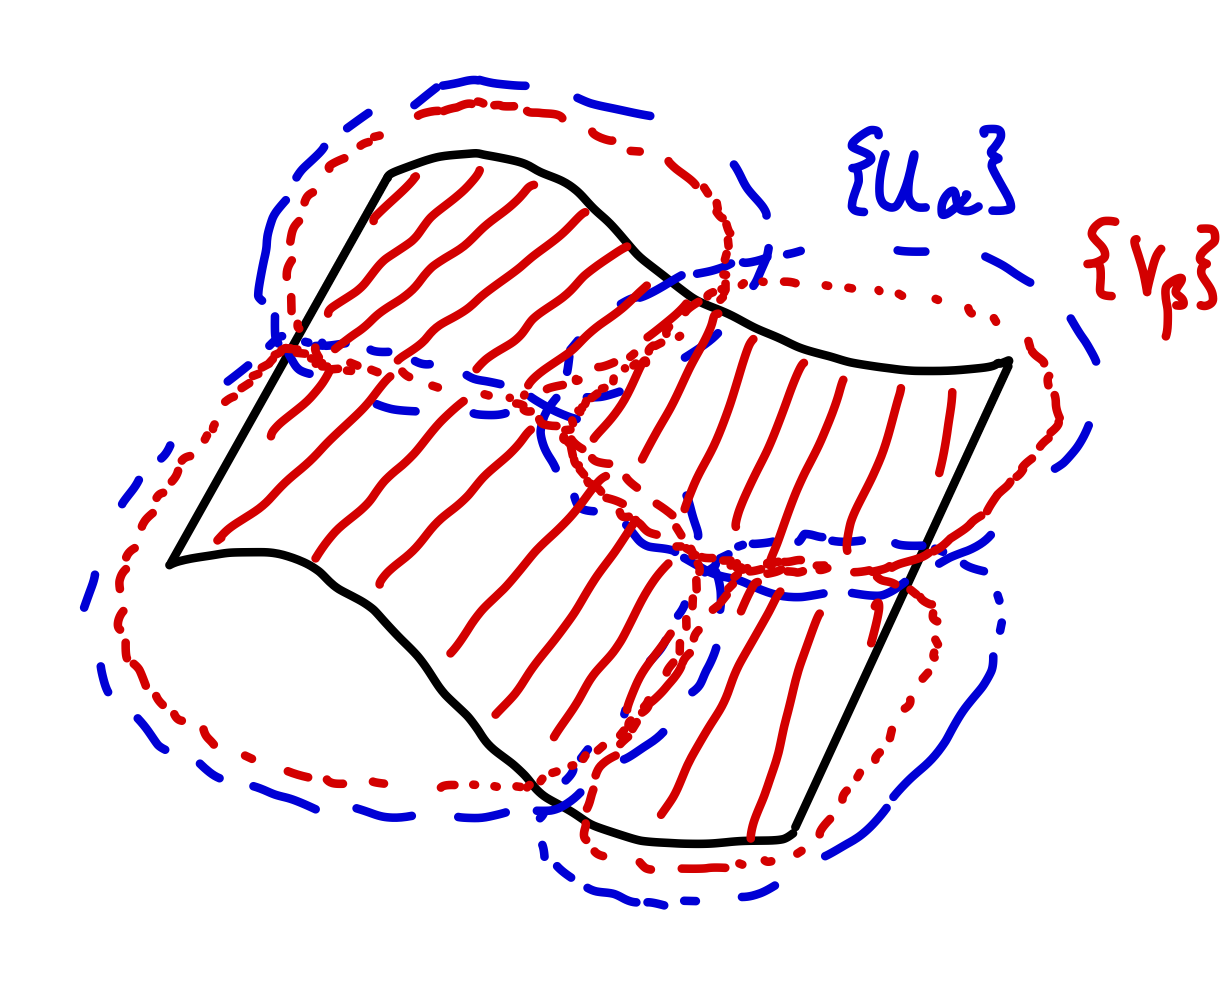
\includegraphics[width=0.2\linewidth]{Bilder/parakompakt.png}
\caption{Eine parakompakte MFK.}
\end{figure}
\end{definition}
\begin{satz}{Parakompaktheit top. MFN}{parakompmfn}
Jede top. MFK ist parakompakt.
\end{satz}
\begin{definition}{\textit{zusammenhängend}}{zusammenhängend}
Sei $\Xs$ ein topologischer Raum. $\Xs$ heißt \textbf{zusammenhängend}, falls er sich nicht in zwei offene, disjunkte, nicht-leere Teilmengen zerlegen lässt.\\
Anders formuliert: Sind $U,V \sub \Xs$ offen, nicht-leer und gilt $X = U \cup V$, so folgt $U \cap V \neq \emptyset$.
\end{definition}
\begin{definition}{\textit{wegzusammenhängend}}{wegzusammenhängend}
Ein topologischer Raum $\Xs$ heißt \textbf{wegzusammenhängend}, falls zu je zwei Punkten $x,y \in X$ eine stetige Abbildung
\begin{equation}
c: [0,1] \to \Xs
\end{equation}
mit $c(0)=x$ und $c(1)=y$ existiert.
\end{definition}
\subsection{Glatte Mannigfaltigkeiten}
\label{subsec: smoothmfn}
\begin{definition}{Karte}{karte}
Sei $X$ eine top. MFK.\\
Eine \textbf{Karte um} $p \in X$ ist eine offene Umgebung $U \sub X$ von $p$ und eine Abbildung 
\begin{equation}
\phi: U \to \R^n,
\end{equation}
die $U$ \textit{homöomorph} auf eine offene Teilmenge $V \in \R^n$ abbildet.
\end{definition}
\begin{definition}{(glatter) Atlas}{atlas}
Sei $X$ eine top. MFK.\\
Unter einem \textbf{Atlas von} $X$ versteht man eine Familie von Karten $(\phi_\alpha, U_\alpha)_{\alpha \in A}$ mit $\bigcup_{\alpha \in A} U_\alpha = X$.\\
Ein Atlas heißt \textbf{glatt}, wenn die Kartenwechselabbildungen glatte Abbildungen zwischen offenen Teilmengen des $\R^n$ sind.
\begin{figure}[H]
\label{fig:kartenwechsel}
\centering
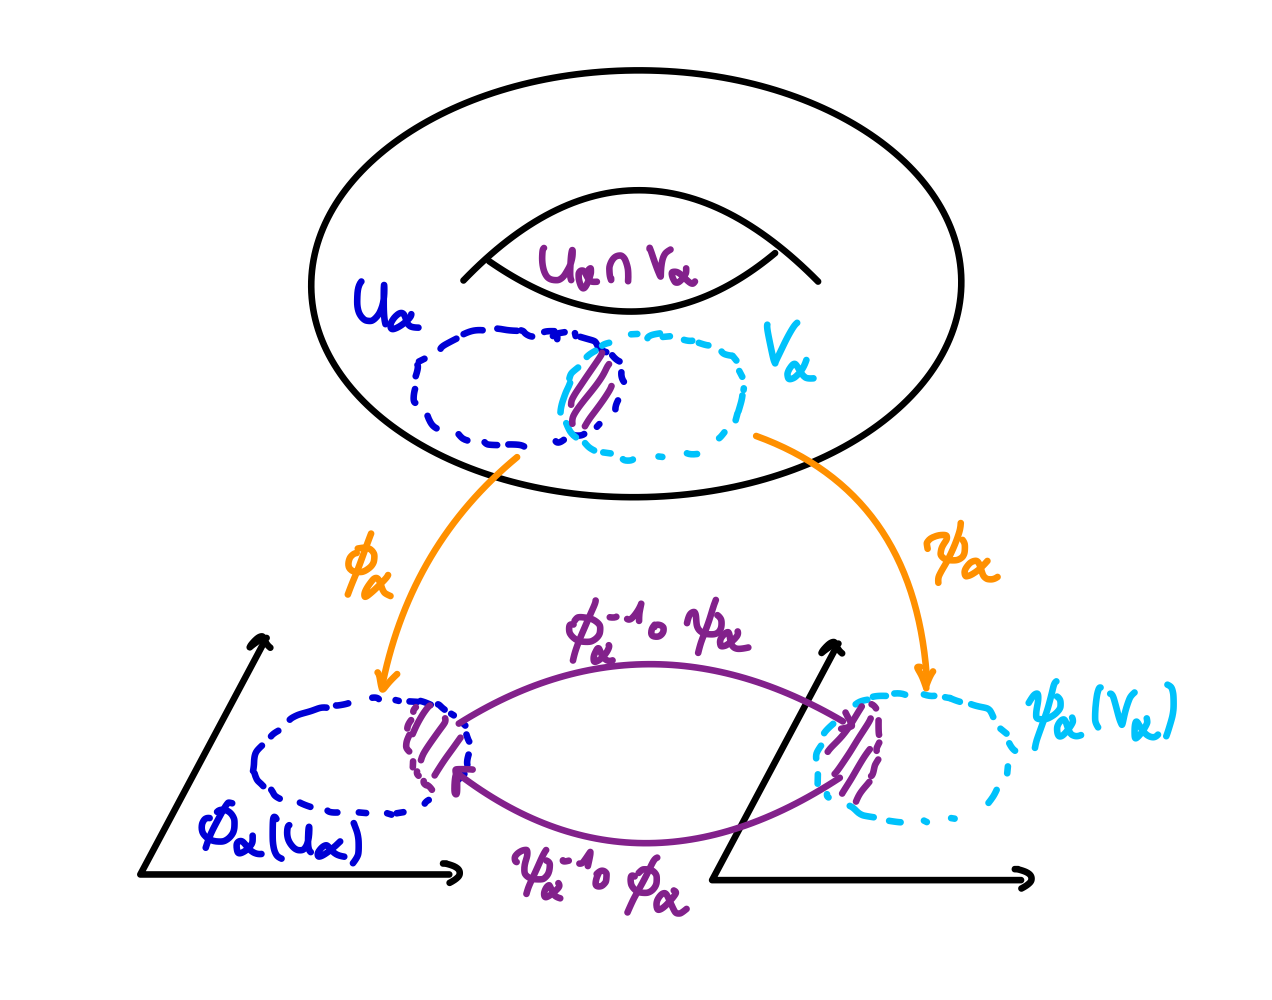
\includegraphics[width=0.3\linewidth]{Bilder/kartenwechsel.png}
\caption{Ein Atlas mit Kartenwechselabbildung.}
\end{figure}
\end{definition}
Wir sehen uns ein Beispiel anhand der schon bekannten $n$-Sphäre an:
\begin{beispiel}{Stereographische Projektion} \\
Sei $X := \sph^n \sub \R^{n+1} \cong \R^n \times \R$. Wir definieren die \textbf{stereographische Projektion} durch:
\begin{align}
\sigma_\pm : \sph^n \exc (0, 0, \dots, \pm 1) & \to \R^n \\
(x_1, \dots, x_{n+1}) & \mapsto \left( \frac{x_1}{1 \mp x_{n+1}}, \dots , \frac{x_n}{1 \mp x_{n+1}} \right)
\end{align} 
Nachrechnen zeigt, dass die Umkehrabbildungen in der Tat durch
\begin{align}
\phi_\pm : \R^n &\to \sph^n \\
y &\mapsto \left( \frac{2y}{1+||y||^2}, \pm \frac{||y||^2 - 1}{||y||^2 + 1}\right)
\end{align}
gegeben sind. Die Kartenübergänge
\begin{equation}
\sigma_\mp \circ \phi_\pm: \R^n \exc \{0\} \to \R^n \exc \{0\} 
\end{equation}
sind durch $y \mapsto \frac{y}{||y||^2}$ gegeben.\\
Auch andere Karten sind möglich:
Betrachte $U_i^\pm := \{ x \in \sph^n | x_i \gtrless 0 \}$ und 
\begin{align}
\psi_i^\pm: U_i^\pm &\to \R^n \\
(x_1, \dots, x_{n+1}) &\mapsto (x_1, \dots, \hat{x}_i, \dots, x_n)
\end{align}
mit Umkehrabbildung:
\begin{align}
\left( \psi_i^\pm \right)^{-1}: \D^n &\to \sph^n \\
(y_1, \dots, y_{n}) &\mapsto (y_1, \dots, y_{i-1}, \pm \sqrt{1-||y||^2}, y_i, \dots, y_n).
\end{align}
\begin{figure}[H]
\label{fig:sphere}
\centering
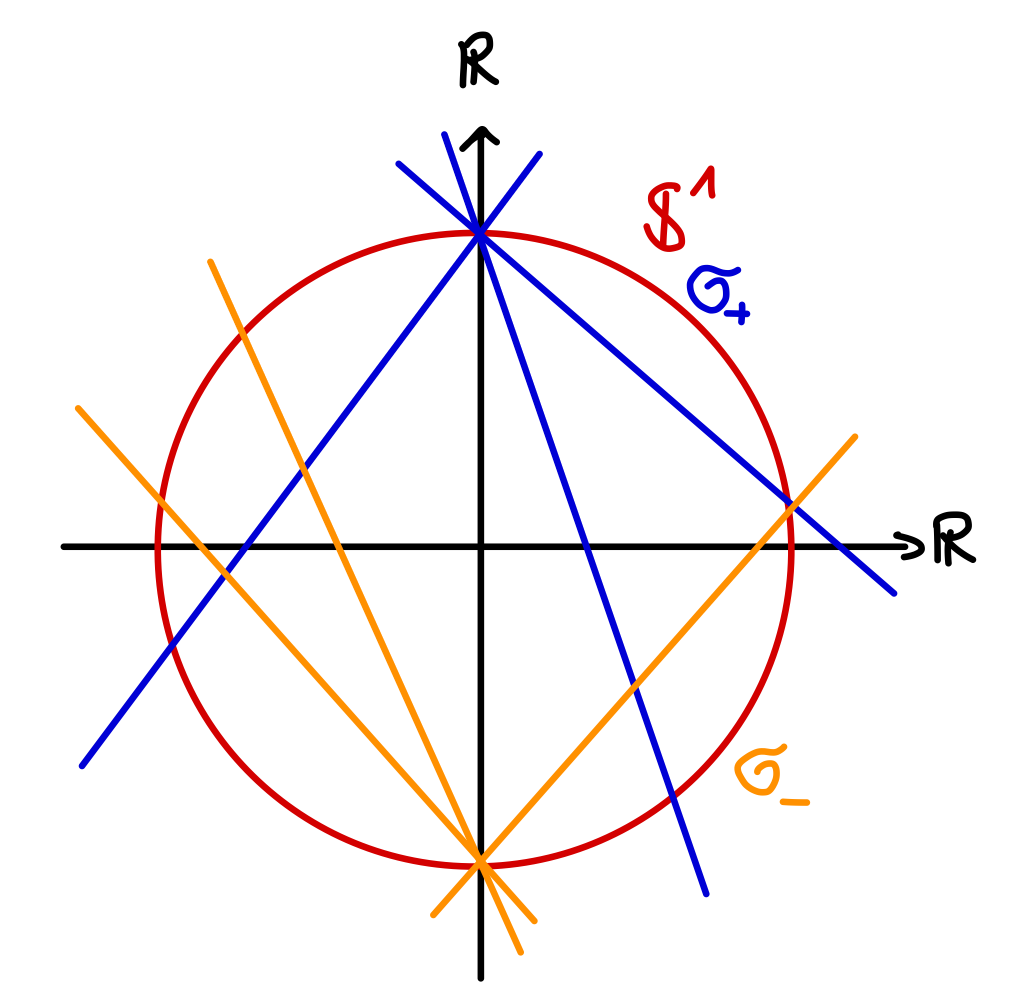
\includegraphics[width=0.2\linewidth]{Bilder/stereograph.png}
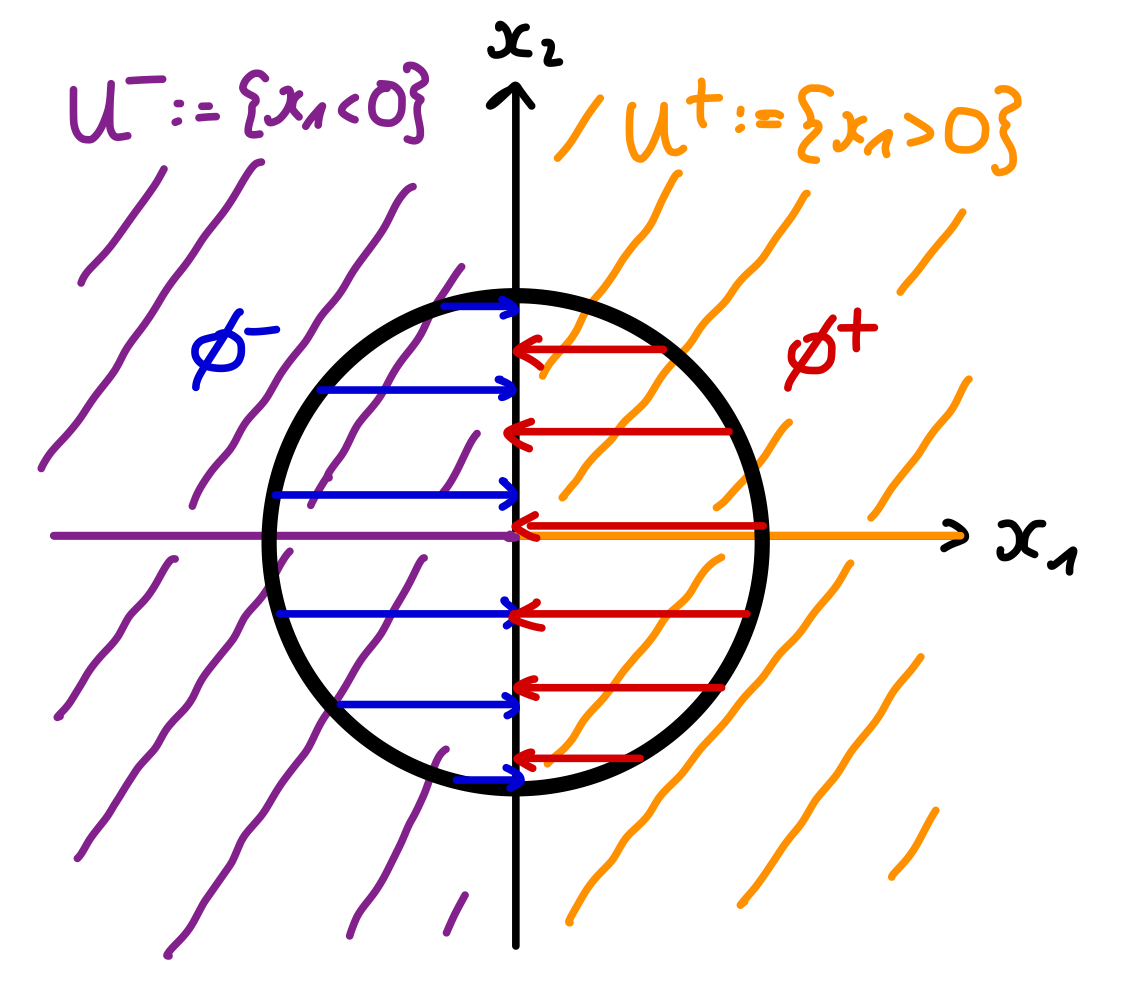
\includegraphics[width=0.2\linewidth]{Bilder/sphereproj.png}
\caption{Zwei Karten für $\sph^2$.}
\end{figure}
\end{beispiel}
\begin{definition}{äquivalente Atlanten}{äquivat}
Sei $X$ eine top. MFK. Zwei glatte Atlanten $\Af_1$ und $\Af_2$ heißen \textbf{äquivalent}, in Zeichen $\Af_1 \sim \Af_2$, wenn die Vereinigung $\Af_1 \cup \Af_2$ auch ein glatter Atlas ist.
\end{definition}
\begin{definition}{glatte Mannigfaltigkeit}{glattmfn}
Eine \textbf{glatte Struktur} auf einer top. MFK $X$ ist eine Äquivalenzklasse glatter Atlanten.\\
Eine \textbf{glatte MFK} ist eine top. MFK mit einer gewählten glatten Struktur.
\end{definition}
\begin{bemerkung}
Die für $\sph^n$ betrachteten Atlanten sind äquivalent, beschreiben also die gleiche glatte Struktur.
\end{bemerkung}
Wir betrachten dafür einige Beispiele:
\begin{beispiele} Einige glatte Strukturen
\begin{enumerate}
\item Die Karte $\id_{\R^n}: \R^n \to \R^n$ macht den $\R^n$ zu einer glatten MFK.
\item Offene Teilmengen von glatten MFKn sind wieder glatte MFKn, da sie die glatte Struktur der umgebenden MFK erben. Sei $O \sub M$ offen und $\phi: U \to \R^n$ eine Karte für $M$. Dann ist $\phi |_{O \cap U}: O \cap U \to \R^n$ eine Karte für $O$.
\item Betrachte $\text{GL}(n, \R) \sub \text{Mat}(n, \R) \cong R^{n^2}$. Als Urbild von $\R \exc \{ 0 \} \sub \R$ unter $\text{det}: \text{Mat}(n, \R) \to \R$ ist $\text{GL}(n, \R)$ offen in $\text{Mat}(n, \R)$.
\item Jede $k$-dim. UMF des $\R^n$ ist eine glatte $k$-dim. MFK.
\item Seien $M_1$ und $M_2$ glatte MFK. Dann ist das Produkt $M_1 \times M_2$ wieder eine glatte MFK. Betrachte dazu Karten $\phi_{1,2}: U_{1,2} \to \R^{n_{1,2}}$ von $M_1$ respektive $M_2$. Dann ist $\phi_1 \times \phi_2: U_1 \times U_2 \to \R^{n_1 + n_2}$ eine Karte für $M_1 \times M_2$.
\end{enumerate}
\end{beispiele}
\begin{bemerkung}Andere Definition glatter MFK \\
Sei $X$ eine Menge und seien $U_\alpha \sub X$ endlich viele Teilmengen mit $\bigcup_\alpha U_\alpha = X$. Seien $\phi_\alpha : U_\alpha \to V_\alpha \sub \R^n$ Bijektionen. Dann definieren wir eine Topologie wie folgt: $U \in X$ ist offen genau dann, wenn $\forall \alpha \in A: \phi_\alpha (U \cap U_\alpha) \sub \R^n$ offen sind.\\
Ist diese Topologie hausdorffsch, ist $X$ eine top. MFK. Sind die Kartenübergänge glatt, erhalten wir die Struktur einer glatten MFK auf X.
\begin{figure}[H]
\label{fig:glattetopmfk}
\centering
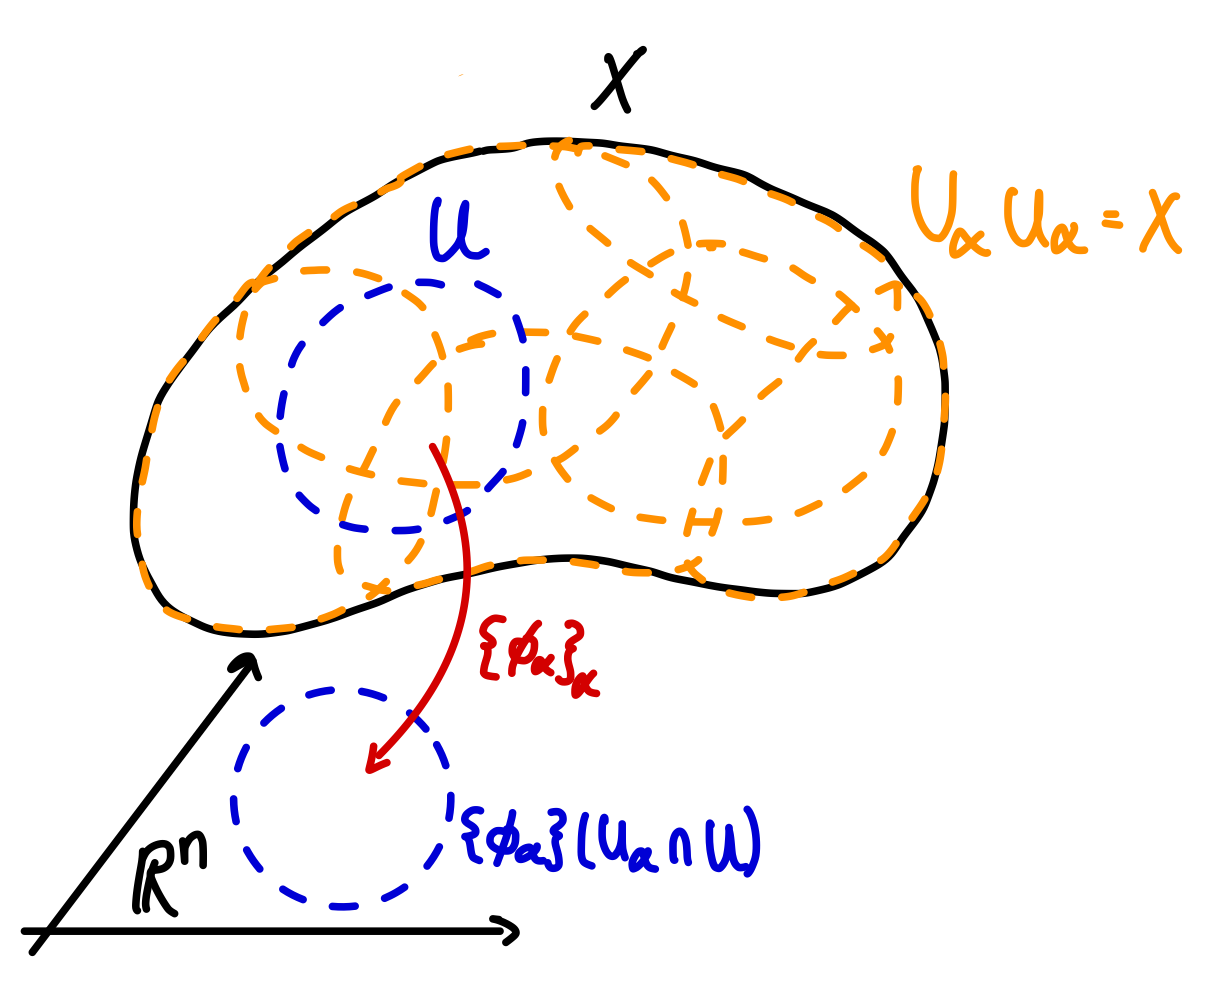
\includegraphics[width=0.25\linewidth]{Bilder/glattetopmfk.png}
\caption{Eine topologische MFK mit Karte in der von den Karten induzierten Topologie.}
\end{figure}
\end{bemerkung}
\begin{beispiel}Der reell projektive Raum \\
Der \textbf{reell projektive Raum} $\R P^n$ besteht aus allen Ursprungsgeraden im $\R^{n+1}$.\\
Für $l \in \R P^n$ betrachten wir 
\begin{align}
U_l :=& \{ g \in \R P^n | \pi_{l|g}: g \to l \ \text{ist ein Isomorphismus} \}\\
=& \{ g \in \R P^n | g \nsubseteq l^\perp \}
\end{align}
Damit ist jede Gerade $g \in U_l$ Graph einer linearen Abbildung $A_g: l \to l^\perp$. Damit bekommen wir die Bijektion $\phi_l : U_l \to L(l, l^\perp) \cong L(\R, \R^n) \cong \R^n$. Der $\R P^n$ erhält so eine Überdeckung durch $\{U_i\}_{i=1}^{n+1}$ mit $U_i \equiv U_{\R_{l_i}}$.
\begin{figure}[H]
\label{fig:sphere}
\centering
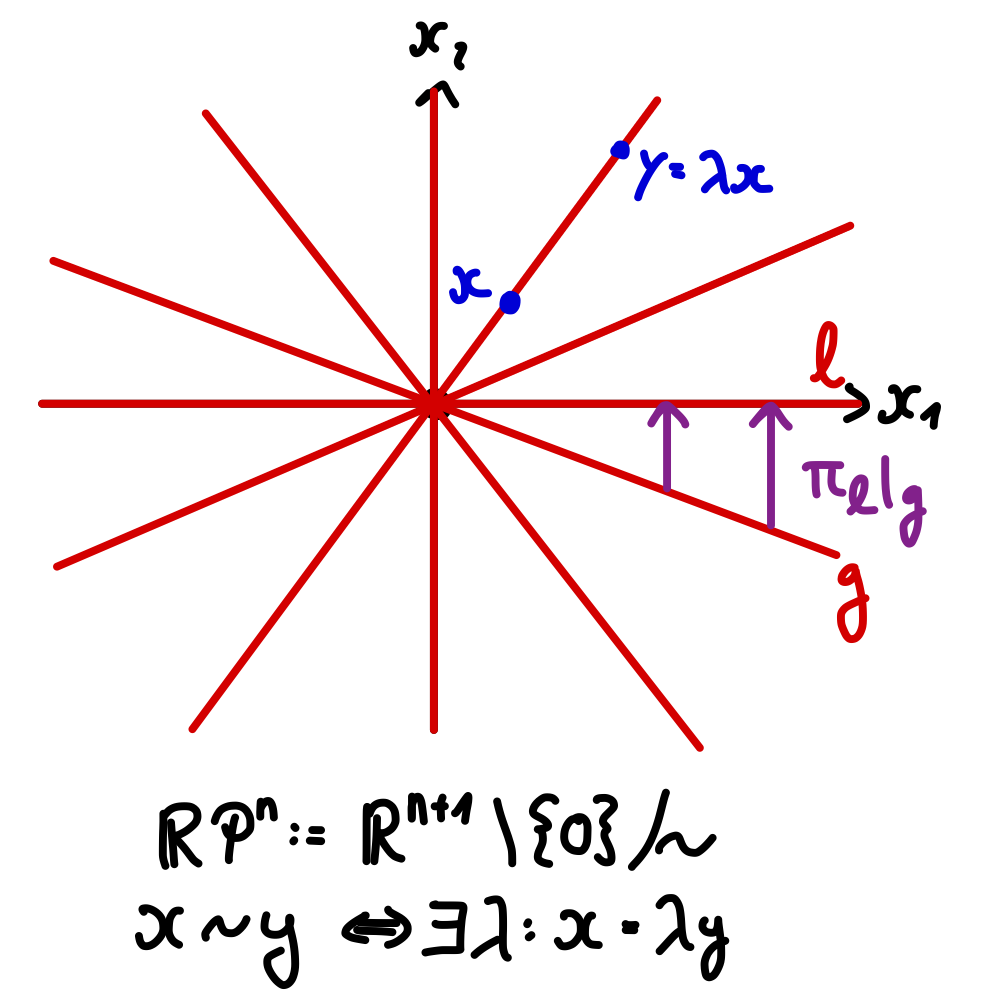
\includegraphics[width=0.25\linewidth]{Bilder/rpn.png}
\caption{Zu sehen ist der $\R P^1$. Die Graphik zeigt, warum man keinen Isomorphismus findet, wenn $l \perp g$ ist: Alle Punkte auf $l$ würden auf einen Punkt auf $g$ abgebildet werden.}
\end{figure}
\end{beispiel}
\begin{satz}{Glatter Atlas für $\R P^n$}{rpnglatt}
Seien $\phi_i$ und $U_i$ wie oben. Dann ist $\Af = \{ (\phi_i, U_i) | 1 \leq i \leq n+1 \}$ ein glatter Atlas für $\R P^n$.
\end{satz}
\begin{beweis}
Bezüglich der Standardkoordinaten ist die Abbildung gegeben durch
\begin{align}
\phi_i : U_i & \to \R^n \\
\R v & \mapsto \left( \frac{v_1}{v_i}, \dots, \hat{\frac{v_i}{v_i}}, \dots, \frac{v_{n+1}}{v_i}\right)
\end{align}
mit der Umkehrabbildung
\begin{align}
\phi_i^{-1}: \R^n &\to U_i \sub \R P^n \\
(y_1, \dots, y_n) &\mapsto \R \cdot (y_1, \dots, y_{i-1}, 1, y_i, \dots, y_n)
\end{align}
Ein Kartenübergang $\phi_j \circ \phi_i ^{-1} : \phi_i (U_i \cap U_j) \to \phi_j (U_i \cap U_j)$ hat dann für $j < i$ die Gestalt:
\begin{align}
\phi_i (U_i \cap U_j) &= \{ y \in \R^n | y_j \neq 0 \} \\
\phi_j (U_i \cap U_j) &= \{z \in \R^n | z_{i-1} \neq 0 \}
\end{align}
Für den Kartenübergang findet man:
\begin{equation}
\phi_j \circ \phi_i^{-1} (y_1, \dots, y_n) = \phi_j (y_1, \dots, y_{i-1}, 1, y_i, \dots, y_n) = \left(\frac{y_1}{y_j}, \dots, \hat{\frac{y_i}{y_j}},\dots, \frac{y_{i-1}}{y_j}, \frac{1}{y_j}, \frac{y_{i}}{y_j}, \dots, \frac{y_{n}}{y_j} \right)
\end{equation}
Da auf dem Definitionsbereich $y_j \neq 0$ gilt, ist der Kartenübergang und damit auch $\Af$ glatt.
\end{beweis}
\begin{korollar}{}{}
Mit den obigen Karten ist $\R P^n$ eine \textit{glatte MFK}.
\end{korollar}
\begin{bemerkung}Grassman-MFK\\
Die Unterräume $G_{k, n} := \{ k \text{-dim. linearer UR des} \ \R^n \}$ erhalten auf analoge Weise die Struktur einer MFK und werden \textbf{Grassman-Mannigfaltigkeiten} genannt.
\end{bemerkung}
Sei $M$ eine top. MFK. Für Dimensionen $n \leq 3$ gibt es für $M$ immer eine eindeutige glatte Struktur. Ab Dimension $n > 3$ ist dies nicht mehr gegeben.
\begin{definition}{glatte Abbildung}{glattfkt}
Seien $M_1$ und $M_2$ glatte MFKn. Eine Abbildung $f: M_1 \to M_2$ heißt \textbf{glatt}, wenn $f$ stetig ist und für alle Karten $(\phi, U)$ von $M_1$ und $(\psi, V)$ von $M_2$ mit $f^{-1}(V) \cap U \neq \emptyset$ die Abbildung
\begin{equation}
\psi \circ f \circ \phi^{-1}: \phi(f^{-1}(V) \cap U) \to \psi (V)
\end{equation}
eine glatte Abbildung zwischen offenen Teilmengen des $\R^{n_1}$ und $\R^{n_2}$ ist.
\begin{figure}[H]
\label{fig:sphere}
\centering
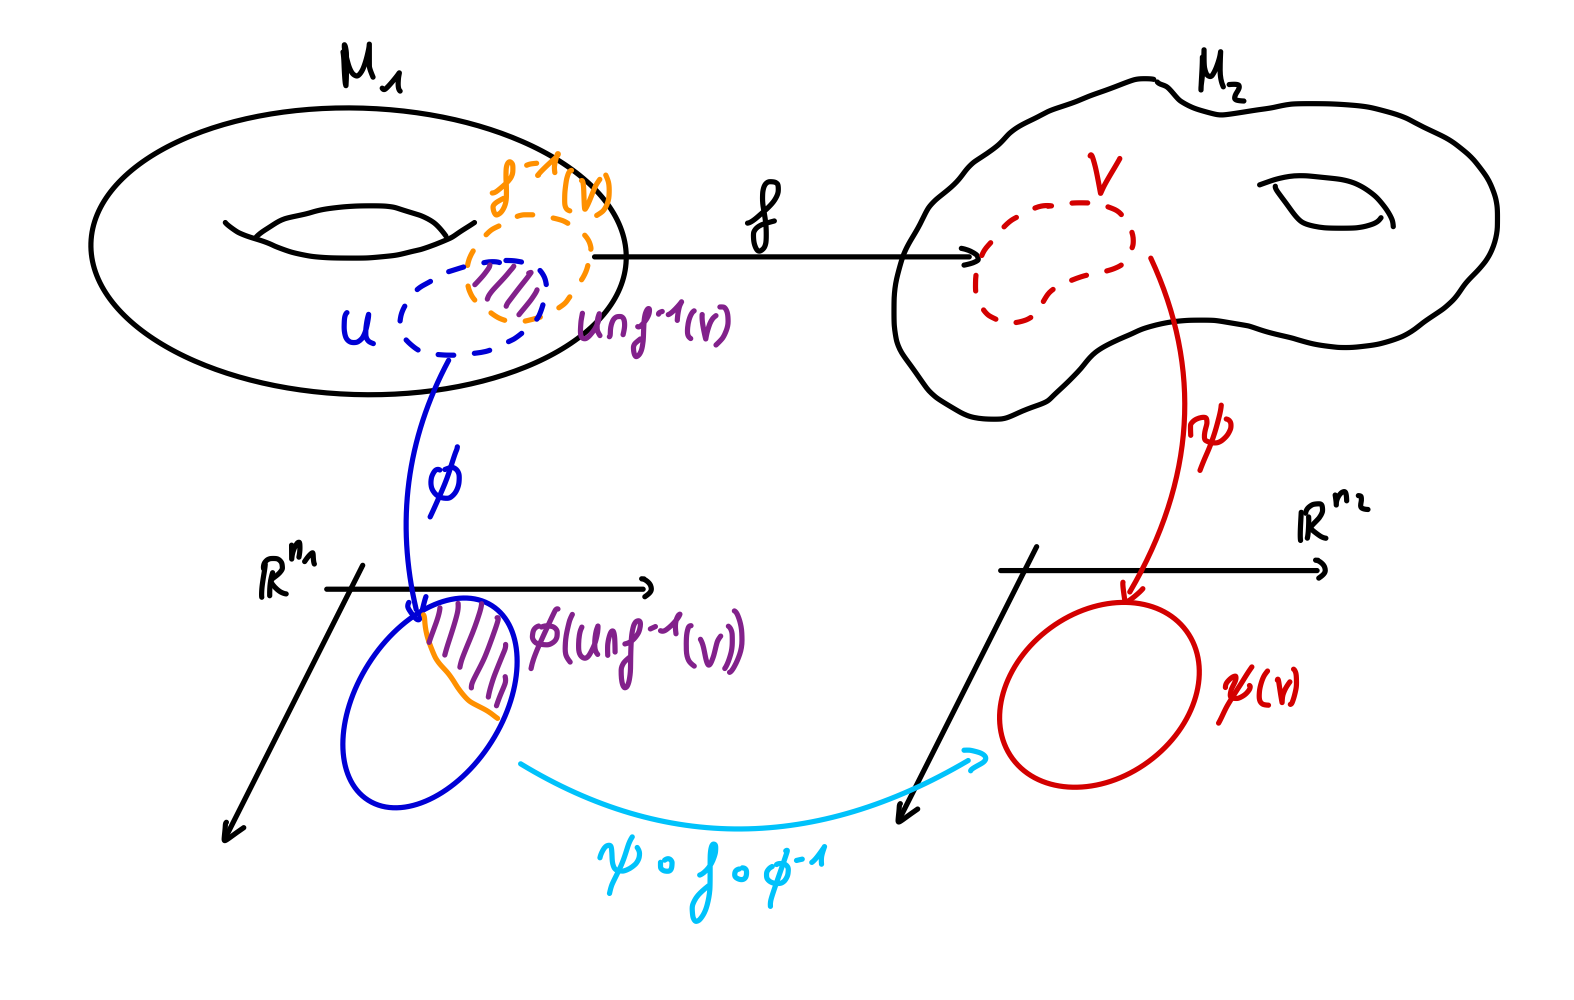
\includegraphics[width=0.3\linewidth]{Bilder/glatteabb.png}
\caption{Kartenwechsel mit einer glatten Abbildung.}
\end{figure}
\end{definition}
\begin{bemerkungen}Spezialfälle glatter Abbildungen\\
\begin{enumerate}
\item Eine Funktion $f: M \to \R$ ist glatt, wenn für alle Karten die Abbildung $f \circ \phi^{-1}: \phi(U) \to \R$ glatt ist.
\item Ist $M \sub \R^n$ eine UMF, so ist $f: M \to \R^k$ genau dann glatt, wenn es zu jedem Punkt $p \in M$ eine offene Umgebung $U \sub \R^n$ und eine glatte Funktion $F: U \to \R^k$ gibt, sodass $f|_{U \cap M} = F|_{U \cap M}$ ist.
\end{enumerate}
\end{bemerkungen}
\begin{definition}{(glatter) Diffeomorphismus}{diffeomorph}
Eine glatte Abbildung $f: M_1 \to M_2$ zwischen glatten MFK $M_1, M_2$ heißt \textbf{(glatter) Diffeomorphismus}, falls gilt:
\begin{itemize}
\item $f$ ist bijektiv.
\item Die Umkehrabbildung $f^{-1}: M_2 \to M_1$ ist ebenfalls glatt.
\end{itemize}
\end{definition}
Für jede glatte MFK $M$ bilden die Diffeomorphismen $M \to M$ eine Gruppe $\diffm (M)$.
\begin{beispiele}
\begin{enumerate}
\item Die Antipodenabbildung
\begin{align}
A: \sph^n &\to \sph^n \\
p &\mapsto -p
\end{align}
ist ein glatter Diffeomorphismus mit $A^{-1} = A$.
\item Für jede MFK $M$ ist die Abbildung
\begin{align}
S: M \times M &\to M \times M \\
(x, y) &\mapsto (y, x)
\end{align}
ein Diffeomorphismus.
\item Die Exponentialabbildung
\begin{align}
\exp: \R &\to \sph^1\\
t &\mapsto (\cos t, \sin t)
\end{align}
ist glatt und \textit{lokal} ein Diffeomorphismus. Das heißt, dass $\exp$ bei Einschränkung auf ein hinreichend kurzes Intervall (Länge $<2\pi$) ein Diffeomorphismus aufs jeweilige Bild ist.
\end{enumerate}
\end{beispiele}
\begin{definition}{glatte Wirkung}{glattewirk}
Eine \textbf{glatte Wirkung} einer Gruppe $G$ auf einer glatten MFK $M$ ist ein \textit{Gruppenhomomorphismus}
\begin{align}
G &\to \diffm (G)\\
g &\mapsto \phi_g: M \to M
\end{align}
mit $\phi_{g_1} \circ \phi_{g_2} = \phi_{g_1g_2}$ und $\phi_{g^{-1}}=(\phi_g)^{-1}$.
\end{definition}
$G \times M \to M, \ (g, x) \mapsto \phi_g(x)$ soll glatt sein, wenn es sich bei $G$ um eine \textit{Lie-Gruppe} handelt.
\begin{beispiele}glatte Wirkungen \\
\begin{enumerate}
\item Die Gruppe $\Z$ wirkt direkt auf $\R$ durch Translationen: Für $k \in \Z$ betrachten wir $\phi_k: \R \to \R, \ t \mapsto \phi_k(t)=t+k$.
\item Die Gruppe $\so{2}$ wirkt auf $\R^2$, wobei der Einheitskreis $\sph^1 \sub \R^2$ invariant bleibt.\\
Sei $A \in \so{2}$ mit $A \neq \id$ und $G_A \sub \so{2}$ die von $A$ erzeugte Untergruppe. Wir unterscheiden zwei Fälle:
\begin{itemize}
\item $A$ ist eine Drehung um einen Winkel $2 \pi \cdot \frac{p}{q}$ mit $\ggt (p,q) = 1$. Dann ist $G_A$ eine \textit{zyklische} Untergruppe der Ordnung $q$.
\item $A$ ist eine Drehung um ein irrationales Vielfaches von $\pi$. Dann ist die Zuordnung $k \mapsto A^k$ injektiv und jede Bahn ist dicht in $\sph^1$.
\end{itemize}
\end{enumerate}
\end{beispiele}
\begin{definition}{freie Wirkung}{freiewirk}
Eine Gruppenwirkung heißt \textbf{frei}, falls für alle $g \in G$ mit $g \neq e$ der Diffeomorphismus $\phi_g: M \to M$ keine \textit{Fixpunkte} hat.
\end{definition}
Man kann zeigen, dass gilt:
\begin{satz}{glatte Struktur und Wirkung}{glattstrukwirk}
Sei $G$ eine endliche Gruppe, die glatt und frei auf einer glatten MFK $M$ wirkt.\\
Dann hat der Quotientenraum $\quotient{M}{G}$ eine eindeutige glatte Struktur, sodass die Projektion
\begin{equation}
\pi: M \to \quotient{M}{G}
\end{equation}
ein lokaler Diffeomorphismus ist.
\end{satz}
\begin{beispiel}Der Linsenraum\\
Seien $p, q \in \N$ teilerfremd mit $q>1$. Dann wirkt $G=\Z_q$ auf $\sph^3 \sub \C^2$ mit dem Erzeuger 
\begin{equation}
\sigma_{p,q} (z_1, z_2)= \left( \exp\left(\frac{2\pi i}{q}\right)z_1, \exp\left(\frac{2\pi i p}{q} \right)z_2\right).
\end{equation}
Der Quotientenraum heißt \textbf{Linsenraum} $\text{L}(p,q)$.
\end{beispiel}
\subsection{Tangentialräume}
\label{subsec:tangentspace}
Im Folgenden wollen wir mehrere Zugänge zu Tangentialräumen diskutieren.\\
Allgemein ist der Tangentialraum $T_pM$ an eine UMF $M \sub \R^n$ im Punkt $p \in M$ ein affiner Unterraum des $\R^n$, der $M$ an diesem Punkt bestmöglich approximiert. In der Analysis identifizieren wir diesen oft mit dem zugehörigen linearen Unterraum. Wir wollen aber den Fußpunkt weiterhin festhalten. \\
Den Tangentialraum an $\R^n$ im Punkt $p \in \R^n$ schreiben wir als $T_p\R^n := \{(p, \xi) | \xi \in \R^n \}$.
Seien $U \sub \R^n$ und $V \sub \R^m$ offen sowie $f: U \to V$ glatt. Dann kann für $p \in U$ die Ableitung $\diff f_p: \R^n \to \R^m$ als lineare Abbildung
\begin{align}
f_{\ast, p}: T_pU &\to T_{f(p)}V \\
(p, \xi) &\mapsto f_{\ast, p}(p, \xi) = (f(p), \diff f_p(\xi))
\end{align}
auffassen. Die Abbildung $f_{\ast, p}$ heißt \textbf{Differential} oder \textbf{Pushforward von} $f$ \textbf{in} $p$.
\begin{figure}[H]
\label{fig:sphere}
\centering
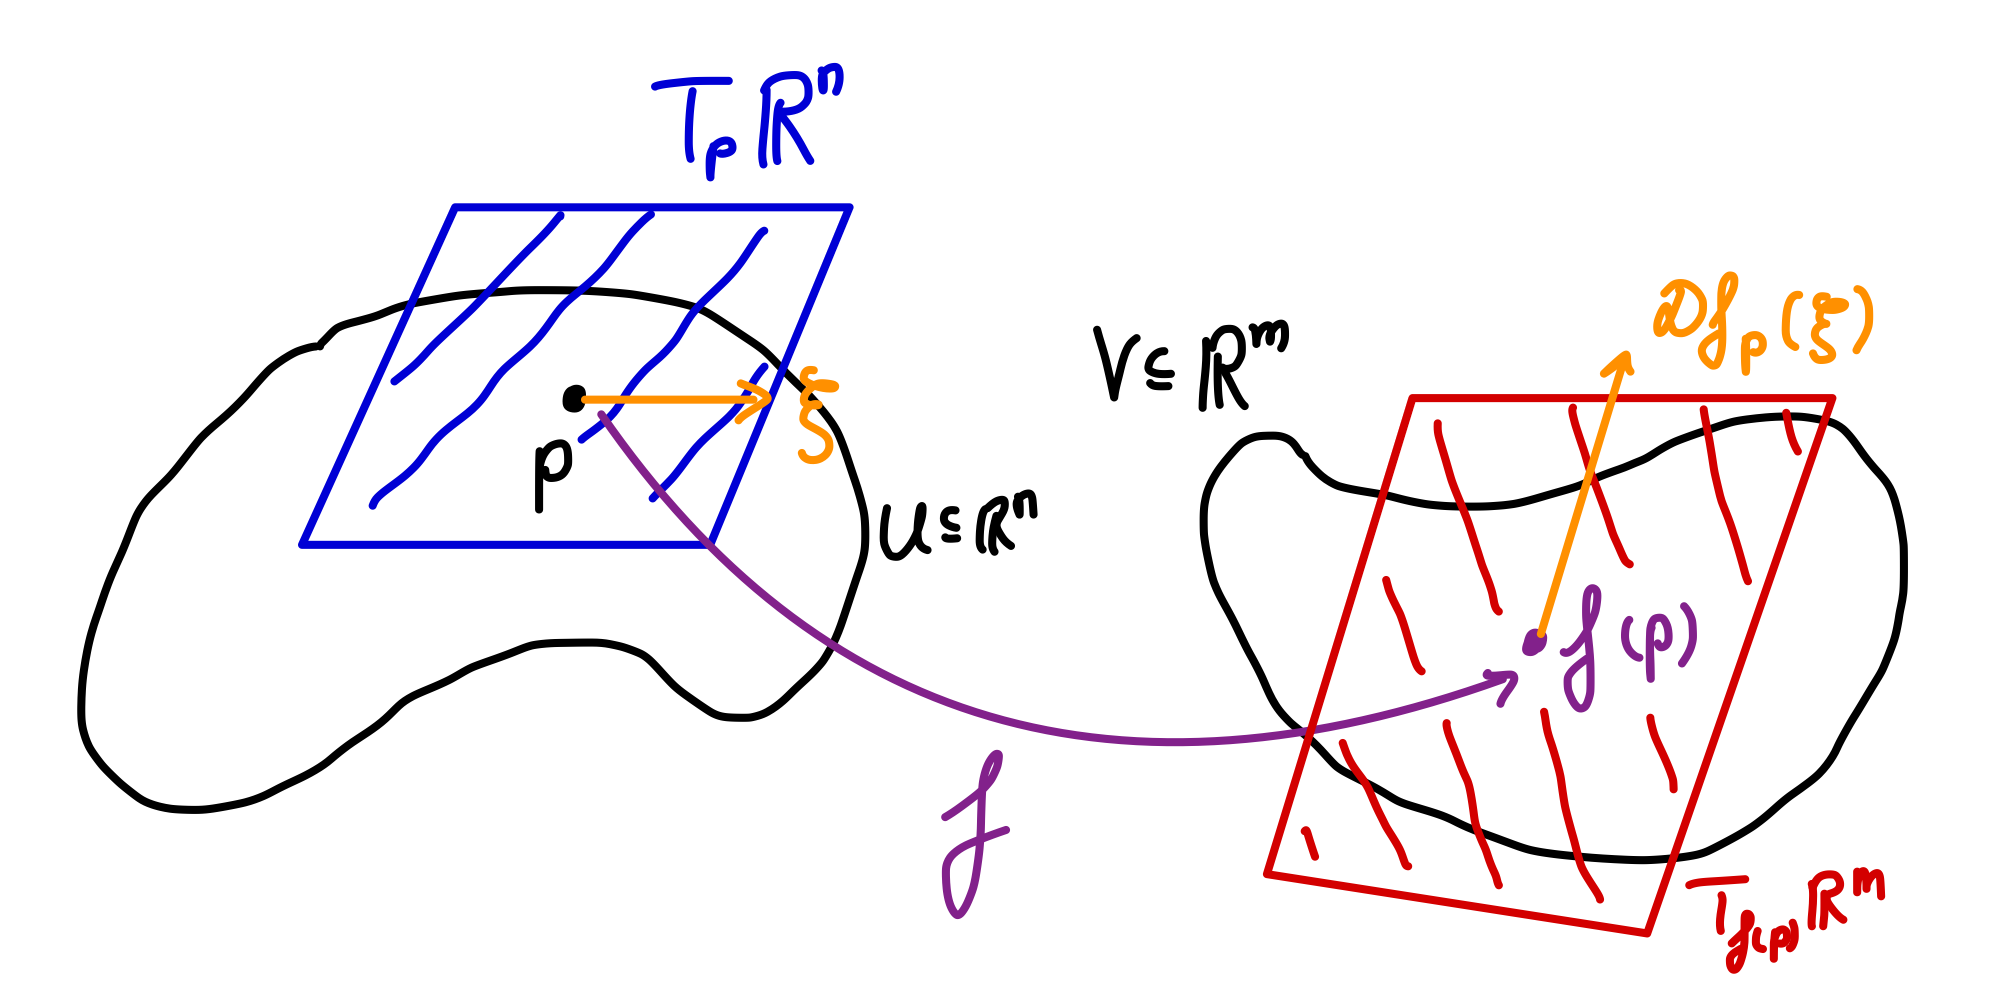
\includegraphics[width=0.3\linewidth]{Bilder/differentialrn.png}
\caption{Das Differential für offene Teilmengen des reellen Raums.}
\end{figure}
\begin{bemerkungen}Kartenwechsel und Differentiale\\
Sei $M$ eine $k$-dim. MFK und $p \in M$. Betrachte die Karten $\phi_1: U_1 \to V_1 \sub \R^k, \ \phi_1(p)=x_1$ und $\phi_2: U_2 \to V_2 \sub \R^k, \ \phi_2(p)=x_2$. Dann ist das Differential des Kartenübergangs
\begin{align}
(\phi_2 \circ \phi_1^{-1})_{\ast, x_1} : T_{x_1}\R^k &\to T_{x_2} \R^k\\
(x_1, \xi) &\mapsto (x_2, \diff (\phi_2 \circ \phi_1^{-1})_{x_1}(\xi))
\end{align}
ein \textit{linearer Isomorphismus}.
\end{bemerkungen}
\begin{definition}{Äquivalenz von Karten}{equivatlant}
Sei $M$ eine glatte MFK durch den Atlas $\Af$. Betrachte
\begin{equation}
\{(\phi, v) | \phi: U \to V \sub \R^k \ \text{ist Karte in} \ \Af \ \text{mit} \ p \in U, v \in T_{\phi(p)}\R^k \}
\end{equation}
mit der Äquivalenzrelation $(\phi, v) \sim_p (\psi, w) \iff w = (\psi \circ \phi^{-1})_{\ast, \phi(p)}(v)$. Transitivität erhalten wir durch die Kettenregel. Zwei Karten heißen \textbf{äquivalent}, wenn sie unter $\sim_p$ äquivalent sind.
\begin{figure}[H]
\label{fig:tangentialvek1}
\centering
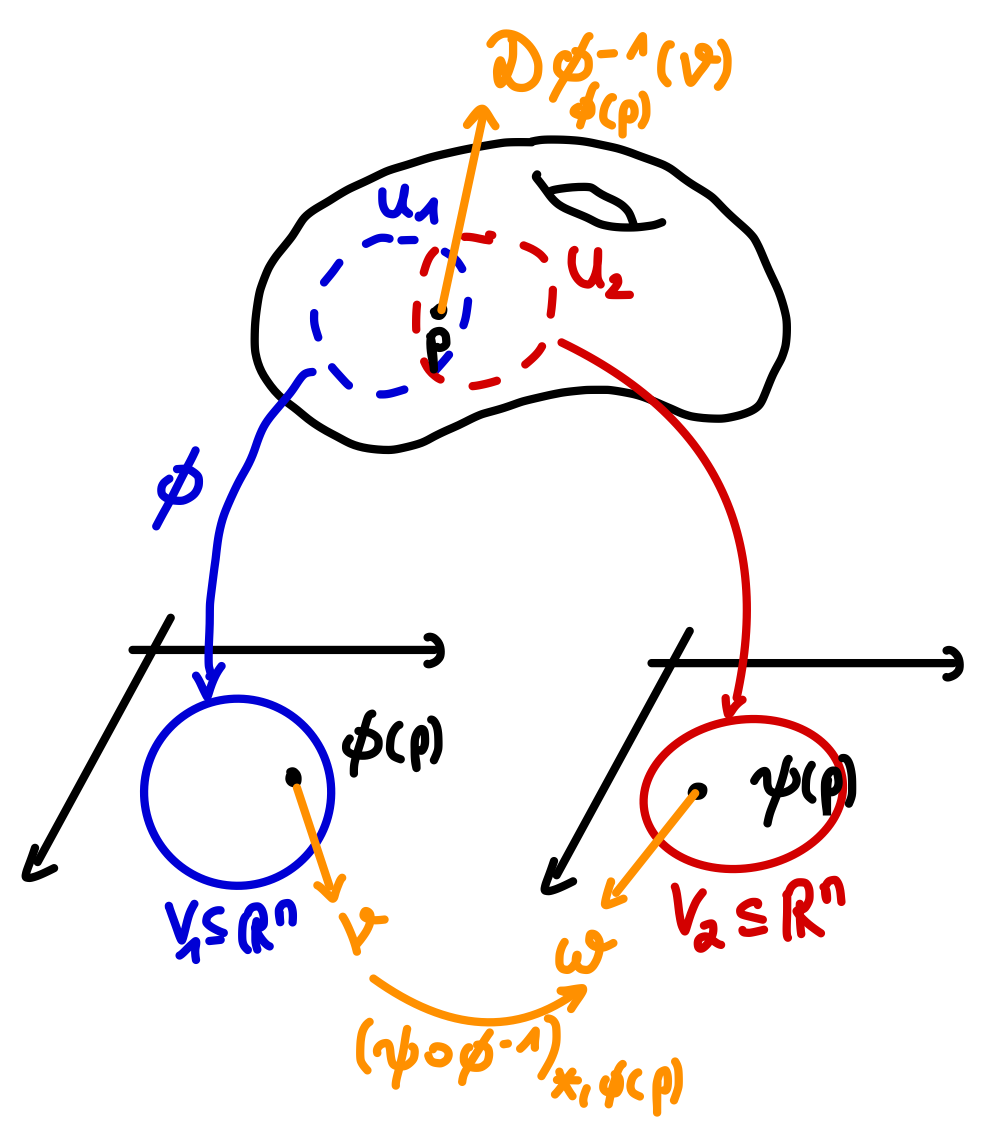
\includegraphics[width=0.2\linewidth]{Bilder/tangentialvek1.png}
\caption{Zwei äquivalente Karten unter $\sim_p$.}
\end{figure}
\end{definition}
\begin{bemerkung}
Für jede Karte $\phi: U \to V \sub \R^k$ in $p$ enthält jede Äquivalenzklasse einen Vertreter der Form $(\phi, v)$.
\end{bemerkung}
Damit kommen wir zu unserer ersten formalen Definition:
\begin{definition}{Tangentialraum (Äquivalenzklasse)}{tangequiv}
Ein \textbf{Tangentialvektor in} $p \in M$ ist eine Äquivalenzklasse der Relation $\sim_p$ Die Menge der Äquivalenzklassen heißt \textbf{Tangentialraum an} $M$ \textbf{in} $p$, geschrieben $T_pM$.
\end{definition}
Versehen mit den Operationen $[(\phi, v)]+[(\phi, w)] := [(\phi, v+w)]$ und $\alpha [(\phi, v)] := [(\phi, \alpha v)]$ wird $T_pM$ ein reeller Vektorraum der Dimension $k$.\\
Daran schließt sich die zweite Definition an:
\begin{definition}{Tangentialraum (Kurven)}{tangkurv}
Betrachte $\{ \gamma: (- \epsilon_\gamma, \epsilon_\gamma) \to M | \gamma \ \text{ist glatt}, \gamma(0)=p \}$ mit der Äquivalenzrelation
\begin{equation}
\gamma_1 \approx_p \gamma_2 \iff \exists \phi: U \to V \ \text{um} \ p \ \text{mit} \ (\phi \circ \gamma_1)'(0) = (\phi \circ \gamma_2)'(0).
\end{equation}
Wegen der Kettenregel stimmen die Tangentialvektoren von $\gamma_1$ und $\gamma_2$ in jeder Karte überein. Die Menge der Äquivalenzklassen sei $\widetilde{T_pM}$. Es gibt eine Bijektion
\begin{align}
\widetilde{T_pM} &\to T_pM \\
[\gamma] &\mapsto [(\phi, (\phi \circ \gamma)'(0))]
\end{align}
für eine feste Karte $\phi: U \to V \sub \R^k$ um $p \in M$, sodass die beiden Definitionen übereinstimmen.
\begin{figure}[H]
\label{fig:tangentialvek2}
\centering
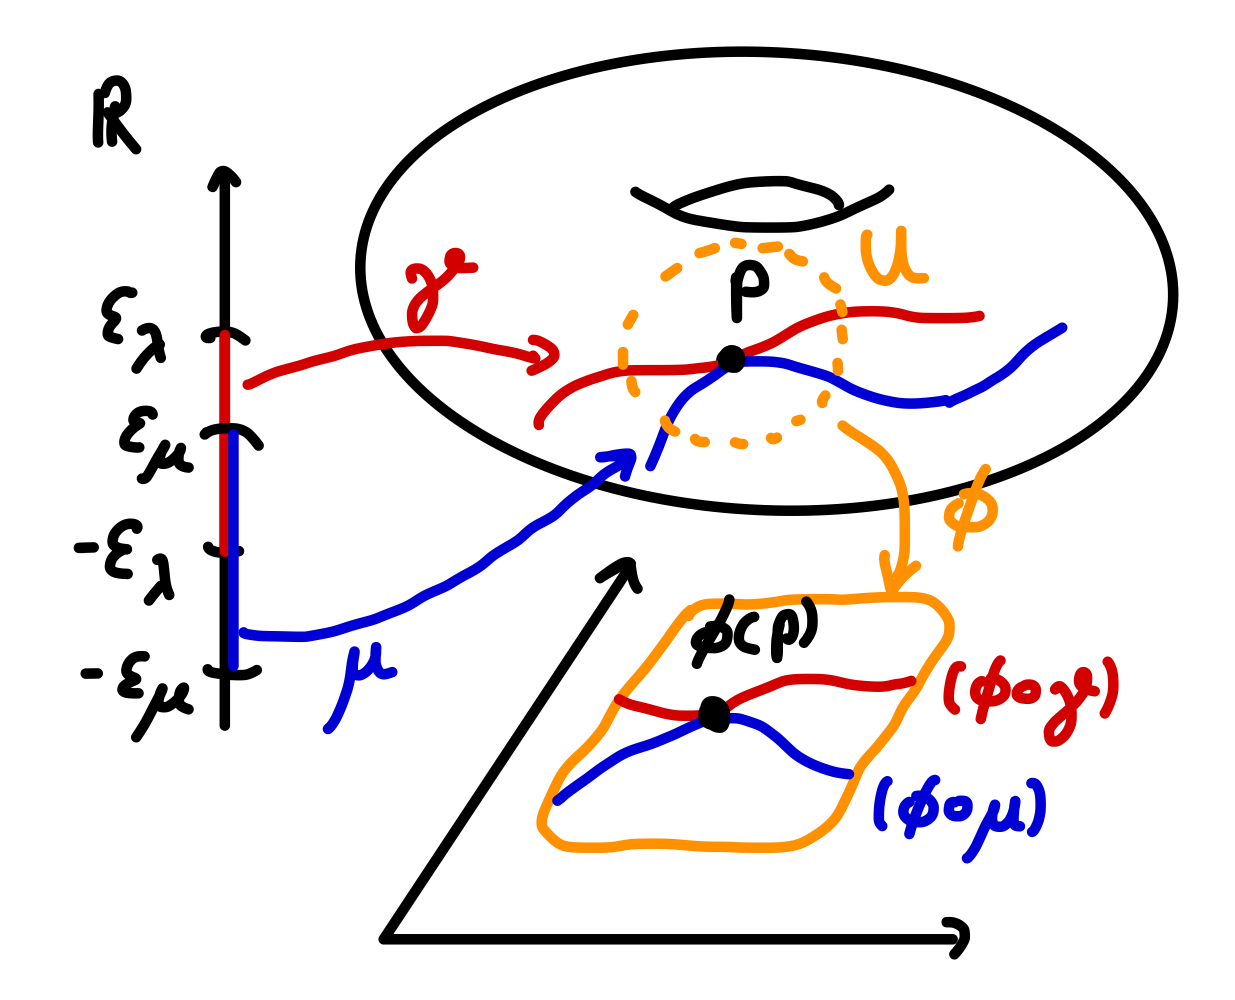
\includegraphics[width=0.2\linewidth]{Bilder/tangentialvek2.png}
\caption{Zwei äquivalente Kurven $\gamma \approx_p \mu$.}
\end{figure}
\end{definition}
Wir entwickeln noch eine dritte Beschreibung.\\
\begin{lemma}{$C^\infty$-Algebra}{}
Sei $C^\infty(M, \R)$ der Vektorraum der glatten Funktionen auf $M$ mit Werten in $\R$. Durch punktweise Multiplikation wird $C^\infty(M, \R)$ zur \textit{Algebra} über $\R$.
\end{lemma}
\begin{definition}{Derivation}{deriv}
Eine \textbf{Derivation} im Punkt $p \in M$ ist eine $\R$-lineare Abbildung
\begin{equation}
\Df: C^\infty(M, \R) \to \R,
\end{equation}
die die \textit{Leibnizregel} $\Df (f \cdot g) = \Df (f) g(p) + f(p) \Df (g)$ erfüllt.\\
Die Menge der Derivationen in $p$ wird mit $\der{p}$ bezeichnet.
\end{definition}
Die Operationen $(\Df_1 + \Df_2)(f) := \Df_1 (f) + \Df_2 (f)$ und $(\alpha \Df)(f) := \alpha \cdot \Df(f)$ machen $\der{p}$ zum reellen VR.
\begin{bemerkung}Konstante Funktionen\\
Für $f(x) \equiv 1$ gilt $f^2 = f$ und damit $\Df (f) = \Df (f^2) = \Df (f) f(p) + f(p) \Df (f)$. Daraus folgt $\Df (f) = 0$. Allgemeiner ist der Wert aller $\Df \in \der{p}$ auf konstanten Funktionen gleich $0$.
\end{bemerkung}
\begin{beispiel}Standardkoordinaten\\
Betrachte $M \sub \R^n$ mit Standardkoordinaten $(x_1, \dots, x_n)$. Die partiellen Ableitungen, ausgewertet in $p \in \R^n$, sind Beispiele für Derivationen in $p$:
\begin{align}
\left.\frac{\partial}{\partial x_i}\right|_p : C^\infty (\R^n, \R) &\to \R \\
f &\mapsto \frac{\partial f}{\partial x_i}(p).
\end{align}
Verallgemeinern lässt sich das wie folgt: Sei $M$ eine glatte MFK und $\phi: U \to V \in \R^k$ eine Karte um $p$ mit Koordinaten $x_i = \pi_i \circ \phi$. Nun definieren wir:
\begin{align}
\left.\frac{\partial}{\partial x_i}\right|_p : C^\infty (M, \R) &\to \R \\
f &\mapsto \frac{\partial (f \circ \phi^{-1})}{\partial x_i}(\phi(p)).
\end{align}
Dies ist eine Derivation in $p \in M$.
\begin{beweis}
Linearität und Leibnizregel sind durch die Ableitungsregeln im $\R^k$ gegeben. Wir zeigen exemplarisch die Leibnizregel:
\begin{align}
\left. \frac{\partial}{\partial x_i}\right|_p (f \cdot g) &= \frac{\partial((f\cdot g)\circ \phi^{-1})}{\partial x_i} (\phi(p)) \\
&= \frac{\partial((f \circ \phi^{-1})( g \circ \phi^{-1}))}{\partial x_i} (\phi(p)) \\
&= \frac{\partial(f \circ \phi^{-1})}{\partial x_i}(\phi(p))\cdot (g \circ \phi^{-1})(\phi (p)) + (f \circ \phi^{-1}) (\phi (p)) \cdot \frac{\partial(g \circ \phi^{-1})}{\partial x_i}(\phi(p)) \\
&=\left.\frac{\partial}{\partial x_i}\right|_p (f) \circ g(p) + f(p) \circ \left.\frac{\partial}{\partial x_i}\right|_p (g)
\end{align}
\end{beweis}
\end{beispiel}
\begin{bemerkung}
Um $\Df \in \der{p}$ auf $f \in C^\infty (M, \R)$ auszuwerten, müssen wir $f$ nur auf einer beliebig kleinen Umgebung von $p$ kennen.
\end{bemerkung}
\begin{satz}{Richtungsableitung}{richtungsabl}
Sei $\phi: U \to V \sub \R^n$ eine Karte um $p \in M$ mit Koordinatenfunktionen $(x_1, \dots, x_n)$. Dann ist die Abbildung 
\begin{align}
T_pM &\to \der{p} \\
[\phi, v] &\mapsto \Df_{[\phi, v]}
\end{align}
mit der Richtungsableitung von $f \circ \phi^{-1}: V \to \R$ in Richtung $v \in T_{\phi(p)}M$, gegeben durch $\Df_{[\phi, v]}(f) = v (f \circ \phi^{-1})$, ein Isomorphismus von $\R$-Vektorräumen.
\begin{figure}[H]
\label{fig:tangentialvek3}
\centering
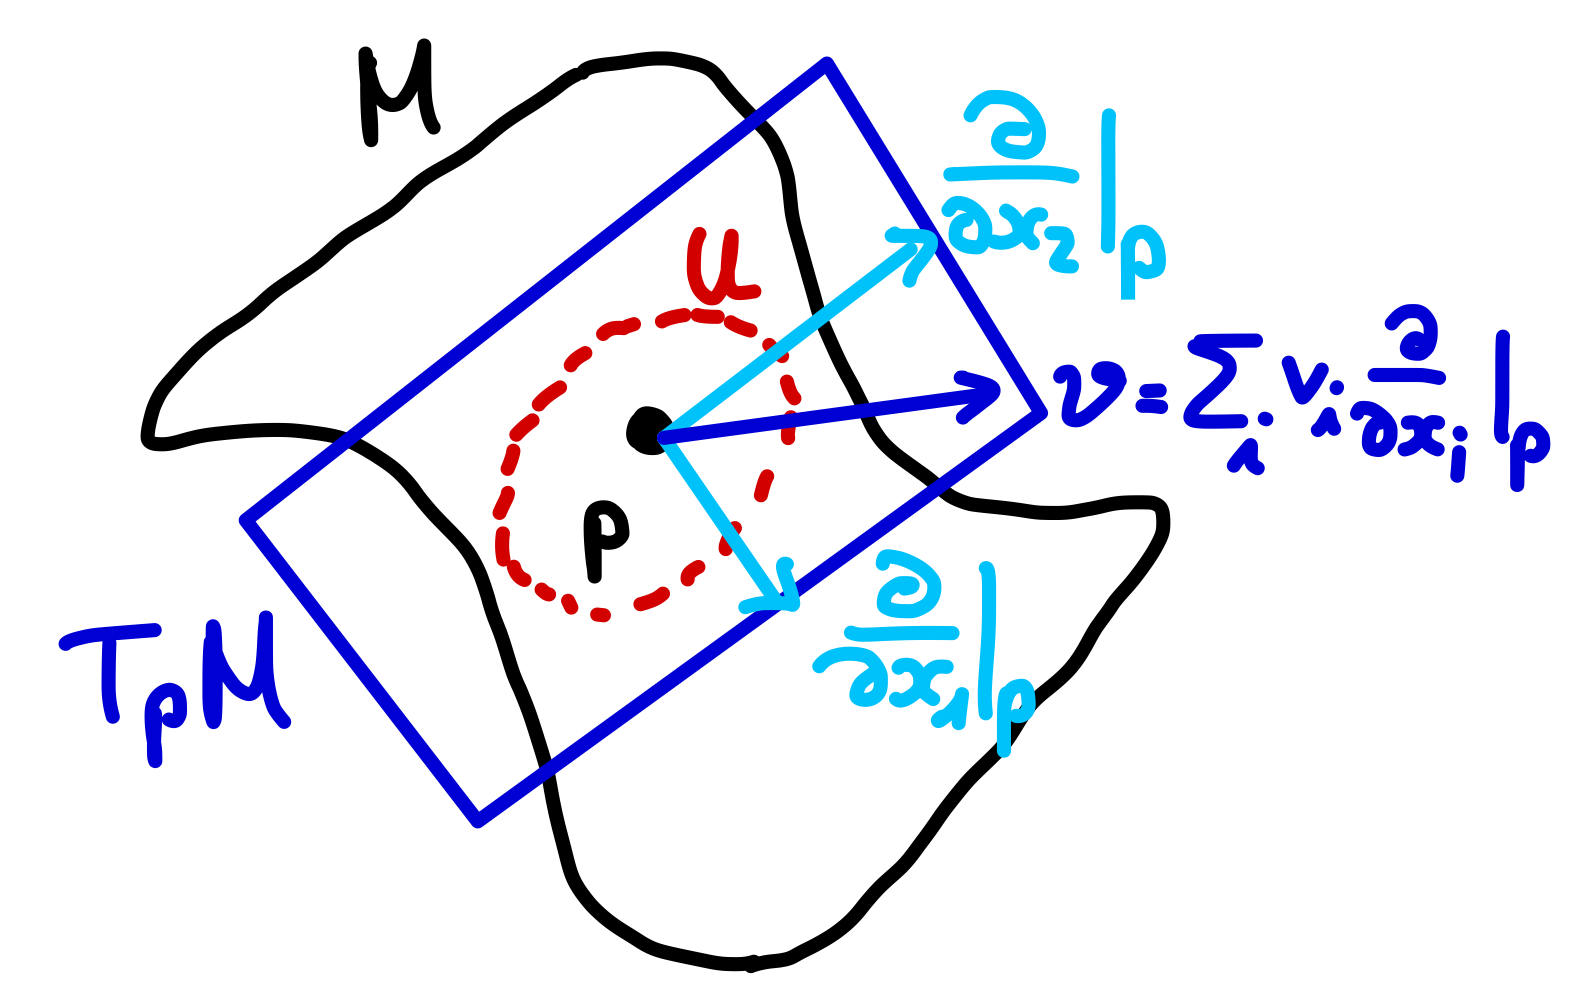
\includegraphics[width=0.2\linewidth]{Bilder/tangentialvek3.png}
\caption{Der von $\frac{\partial}{\partial x_i}$ aufgespannte Tangentialraum an $p$.}
\end{figure}
\end{satz}
\begin{beweis}
Die Abbildung ist durch die Kettenregel wohldefiniert.\\
Der Tangentialvektor $[\phi, (\phi|_p, e_i)]$ wird auf $\left.\frac{\partial}{\partial x_i}\right|_p$ abgebildet. Für die lokal auf $U$ definierten Koordinatenfunktionen $x_j: U \to \R$ gilt aber $\frac{\partial x_j}{\partial x_i} (p) = \delta_{ij}$, also ist die oben definierten Abbildung injektiv. Um zu zeigen, dass sie surjektiv ist, gilt es, zu zeigen, dass\footnote{$\langle \dots \rangle$ steht hier für das Erzeugnis.}
\begin{equation}
\der{p} = \left\langle \left. \frac{\partial}{\partial x_1}\right|_p, \dots, \left. \frac{\partial}{\partial x_n}\right|_p \right\rangle
\end{equation}
\let\qed\relax
\end{beweis}
\begin{lemma}{Taylorentwicklung}{}
Ist $f \in C^\infty (M, \R)$ und $\phi: U \to V \in \R^n$ eine Karte um $p$ mit Koordinaten $(x_1, \dots, x_n)$, dann existiert eine offene Umgebung $W \sub U$ von $p$ und Funktionen $f: W \to \R$, $i \in \{1, \dots, n \}$, sodass $f|_W (q) = f(p) + \Sum{i,1,n} (x_i(q)-x_i(p)) \cdot f_i(q)$.$(\ast)$
\end{lemma}
\begin{beweis}
Sei $W' \sub V = \phi(U)$ eine konvexe Umgebung von $\phi(p)$. Wir schreiben $x_0 := \phi(p)$. Dann gilt für $x \in W'$:
\begin{equation}
(f \circ \phi^{-1})(x)-(f \circ \phi^{-1})(x_0) = \int_0^1 \frac{d}{dt} (f \circ \phi^{-1})(x_0 + t(x-x_0)) dt = \Sum{i,1,n} (x_i - x_i(p)) \underbrace{\int_0^1 \frac{\partial(f \circ \phi^{-1})}{\partial x_i}(x_0 + t(x-x_0))dt}_{=:\tilde{f}_i(x)}
\end{equation}
Mit $W:= \phi^{-1}(W'), q= \phi^{-1}(x)$ und $f_i: W \to \R$, definiert als $\tilde{f}_i \circ \phi$, folgt $(\ast)$. 
\end{beweis}
Weiter mit der Hauptaussage:
\begin{beweis}
Aus $(\ast)$ erhalten wir
\begin{equation}
\left. \frac{\partial}{\partial x_i}\right|_p (f) = \Sum{j,1,n} \left. \frac{\partial}{\partial x_i}\right|_p (x_j - x_j(p)) \cdot f_j] = \Sum{j,1,n} \delta_{ij} \cdot f_j (p) + \cancel{(x_j(p)-x_j(p))} \cdot \left. \frac{\partial}{\partial x_i}\right|_p (f_j) = f_i(p)
\end{equation}
Für eine beliebige Derivation $\Df \in \der{p}$ gilt nun
\begin{equation}
\Df (f) = \Sum{i, 1,n} \Df(x_i - x_i (p)) \cdot f_i = \Sum{i,1,n} \Df(x_i) \cdot f_i(p)+\cancel{(x_i(p)-x_i(p))} \cdot \Df (f_i) = \left( \Sum{i,1,n} \Df (x_i) \left.\frac{\partial}{\partial x_i}\right|_p \right)(f)
\end{equation}
Wir haben also ein beliebiges $\Df \in \der{p}$ als Linearkombination der $\left.\frac{\partial}{\partial x_i}\right|_p$ ausgedrückt.
\end{beweis}
\begin{warning}
Ab jetzt schreiben wir nur $v \in T_pM$ für einen Tangentialvektor in $p \in M$.
\end{warning}
\begin{definition}{Differential}{diff}
Seien $M_1, M_2$ glatte MFK und $F: M_1 \to M_2$ glatte MFK zwischen diesen. Das \textbf{Differential} oder der \textbf{Pushforward} von $F$ im Punkt $p \in M_1$ ist die lineare Abbildung:
\begin{align}
F_{\ast, p}: T_pM_1 &\to T_{F(p)}M_2 \\
v &\mapsto F_{\ast, p} (v)
\end{align}
mit $F_{\ast, p} (v)(f) = v(f \circ F)$ für alle $f \in C^\infty (M_2, \R)$.
\begin{figure}[H]
\label{fig:differential}
\centering
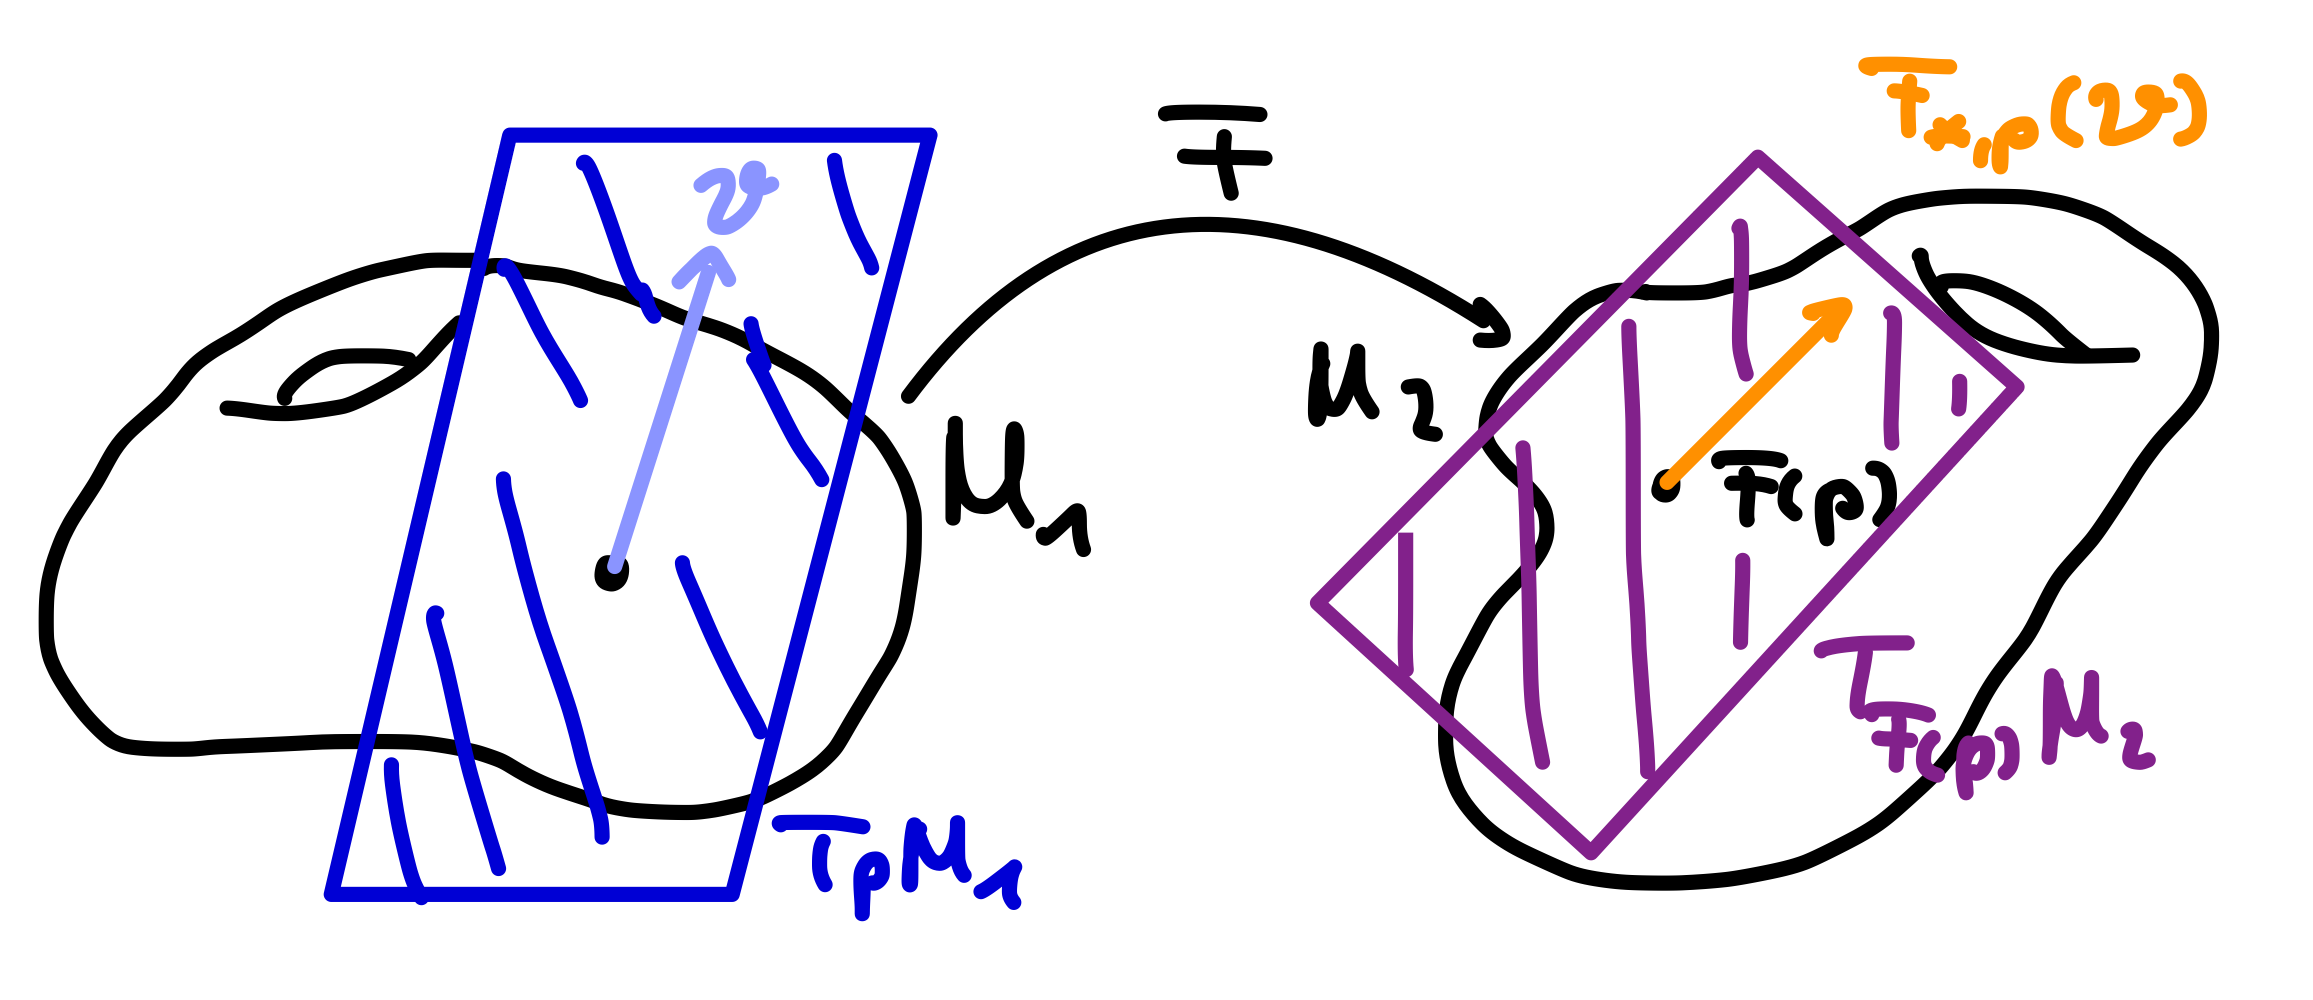
\includegraphics[width=0.3\linewidth]{Bilder/differential.png}
\caption{Dargestellt ist das Differential einer glatten Abbildung $F: M_1 \to M_2$.}
\end{figure}
\end{definition}
\begin{definition}{\textit{lokaler Diffeomorphismus}}{lokalerdiff}
Seien $M,N$ glatte MFKn mit oder ohne Rand. Dann heißt $F: M \to N$ \textbf{lokaler Diffeomorphismus}, wenn alle $p \in M$ eine Umgebung $U \sub M$ haben, sodass $F(U)$ offen in $N$ und $F|_U: U \to F(U)$ ein Diffeomorphismus ist.
\end{definition}
\begin{theorem}{\textit{Umkehrsatz für Mannigfaltigkeiten}}{großerumkehrsatz}
Seien $M,N$ glatte MFKn und sei $F:M \to N$ eine glatte Abbildung. Wenn $F_{\ast, p}$ invertierbar ist in $p \in M$, so existieren zusammenhängende Umgebungen $U_0$ von $p$ und $V_0$ von $F(p)$, sodass
\begin{equation}
F|_{U_0}: U_0 \to V_0
\end{equation}
ein Diffeomorphismus ist.
\end{theorem}
Es gelten die üblichen Rechenregeln, unter anderem die Kettenregel:
\begin{satz}{Kettenregel}{kettenrgl}
Sind $F: M_1 \to M_2$ und $G: M_2 \to M_3$ glatt, so gilt
\begin{equation}
(G \circ F)_{\ast, p} = G_{\ast, F(p)} \circ F_{\ast, p}.
\end{equation}
\end{satz}
\begin{beweis}
Für $f: M_3 \to \R$ gilt 
\begin{equation}
G_{\ast, F(p)} \circ F_{\ast, p} (v)(f) = F_{\ast, p} (v) (f \circ G) = v(f \circ (G \circ F)) = (G \circ F)_{\ast, p} (v)(f).
\end{equation}
\end{beweis}
Für konkrete Rechnungen wollen wir $F_{\ast, p}$ in Koordinaten ausdrücken:\\
Sei dazu $F: M_1 \to M_2$ glatt und $p \in M_1$. Sei $\phi: U \to \R^n$ eine Karte um $p$ mit Koordinaten $(x_1, \dots, x_n)$ und $\psi: W \to \R^m$ eine eine Karte um $F(p)$ mit Koordinaten $(y_1, \dots, y_m)$. Für $w \in T_{F(p)}M_2$ und $f \in C^\infty(M_2)$ gilt dann 
\begin{equation}
w(f) = \Sum{j,1,m} w(y_j) \left.\frac{\partial}{\partial y_j}\right|_{F(p)}(f).
\end{equation} 
Daraus folgt für $v \in T_pM_1$:
\begin{equation}
F_{\ast, p}(v)(f) = \Sum{j,1,m}F_{\ast, p}(v)(y_j) \left.\frac{\partial}{\partial y_j}\right|_{F(p)}(f) = \Sum{j,1,m} v(y_j \circ F) \left.\frac{\partial}{\partial y_j}\right|_{F(p)}(f).
\end{equation}
Die Darstellung $v = \Sum{i,1,n} v_i \left.\frac{\partial}{\partial x_i}\right|_{p}$ liefert
\begin{equation}
F_{\ast, p}(v)(f) = \Sum{i,1,n}\Sum{j,1,m} \frac{\partial (y_i \circ F \circ \phi^{-1})}{\partial x_i} (\phi(p)) \cdot v_i \cdot \left.\frac{\partial}{\partial y_j}\right|_{F(p)}(f).
\end{equation}
Das ist auch gleich der Beweis für:
\begin{satz}{Matrixdarstellung}{mtrx}
In den lokalen Koordinaten $\phi: U \to \R^n$ auf $M_1$ und $\psi: W \to \R^m$ auf $M_2$ hat $F_{\ast, p}: T_pM_1 \to T_{F(p)}M_2$ bezüglich der Basen $\left( \left.\frac{\partial}{\partial x_1}\right|_p, \dots, \left.\frac{\partial}{\partial x_n}\right|_p \right)$ von $T_pM_1$ und $\left( \left.\frac{\partial}{\partial x_1}\right|_{F(p)}, \dots, \left.\frac{\partial}{\partial x_m}\right|_{F(p)} \right)$ von $T_{F(p)}M_2$ die Matrixdarstellung
\begin{equation}
\left\{ \frac{\partial (\psi \circ F \circ \phi^{-1})_j}{\partial x_i} (\phi(p))\right\}_{\substack{j= \{1, \dots, m\}\\i = \{ 1, \dots, n\}}}.
\end{equation}
\end{satz}
\begin{beispiel}
Sei $c: (a,b) \to M$ eine glatte Kurve in $M$. Für $t_0 \in (a,b)$ bezeichnet $\left.\frac{\partial}{\partial t}\right|_{t_0}$ den Standard-Basisvektor von $T_{t_0}\R \cong \R$. Der Tangentialvektor an $c$ in $c(t_0)$ ist dann $c'(t_0)=\dot{c}(t_0):= c_{\ast, t_0}\left(\left.\frac{\partial}{\partial t}\right|_{t_0} \right) \in T_{c(t_0)}M$. Ist $F: M \to N$ eine glatte Abbildung, gilt $F_{\ast, c(t_0)} (c'(t_0)) = (F \circ c)'(t_0) \cdot \left.\frac{\partial}{\partial t}\right|_{F \circ c(t_0)}$.
\end{beispiel}
\begin{definition}{Submersion, Immersion, Einbettung}{subimein}
Eine glatte Abbildung $F: M \to N$ zwischen glatten MFK $M, N$ heißt:
\begin{itemize}
\item \textbf{Immersion}, wenn $F_{\ast, p}: T_pM \to T_{F(p)}N$ für alle $p \in M$ injektiv ist.
\item \textbf{Submersion}, wenn $F_{\ast, p}: T_pM \to T_{F(p)}N$ für alle $p \in M$ surjektiv ist.
\item \textbf{Einbettung}, falls $F$ eine Immersion ist und $F: M \to F(M) \sub N$ ein \textit{Homöomorphismus} ist.
\end{itemize}
\end{definition}
\begin{bemerkung}
Einbettung $\implies$ injektive Immersion, aber injektive Immersion $\xcancel{\implies}$ Einbettung.
\end{bemerkung}
\begin{beispiele} Submersionen, Immersionen und Einbettungen\\
\begin{enumerate}
\item Wir betrachten $F: \R \to \R^2, F(t):=(\sin t, \sin 2t)$. Man rechnet nach, dass $F$ eine Immersion ist. Auf $(0, 2\pi)$ ist $F$ auch injektiv, aber keine Einbettung. Auf $(\epsilon, 2\pi - \epsilon)$ für $\epsilon > 0$ ist $F$ aber eine Einbettung.
\item Sei $M=\Z$ und $N= \sph^1 \cong \quotient{\R}{\Z}$. Für $\alpha \in \R, \Q$ ist die Abbildung $F_\alpha: \Z \to \sph^1, \ k \mapsto k \alpha \mod 1$ eine injektive Immersion, aber keine Einbettung, da $F_\alpha(\Z) \sub \sph^1$ nicht die diskrete Topologie hat.
\item Jede Projektion $\pi: \R^n \to L \sub \R^k$ auf einen linearen UR $L \in \R^n$ entlang des orthogonalen Komplements $L^\perp \sub \R^n$ ist eine Submersion. Jede lineare Einbettung $A: \R^k \to \R^n$ ist eine Immersion.
\item $F: \R^{n+1} \exc \{0\}  \to \R, \ F(x) := ||x||^2$ ist eine Submersion, denn $\Ds F_x(v) = 2 \ip{x,v}$.
\item $G:  \R^{n+1} \exc \{0\} \to \sph^n, \ G(x):=\frac{x}{||x||^2}$ ist auch eine Submersion.
\end{enumerate}
\end{beispiele}
\begin{satz}{\textit{Rangsatz}}{rangsatz}
Seien $M$ und $N$ glatte MFKn mit $m = \dim M$ und $n = \dim N$. Sei weiterhin $F: M \to N$ glatt mit konstantem Rang $r$. Dann existieren für jedes $p \in M$ glatte Karten $(U,\phi)$ von $M$ um $p$ und $(V,\psi)$ von $N$ um $F(p)$, sodass $F(U) \sub V$, in denen $F$ die lokale Koordinatendarstellung 
\begin{equation}
\hat{F} (x_1, \dots, x_r, x_{r+1}, \dots, x_m) = (x_1, \dots, x_r, 0, \dots, 0)
\end{equation}
besitzt.\\
Ist $F$ eine glatte \textcolor{red}{Submersion}, so gilt sogar
\begin{equation}
\hat{F} (x_1, \dots, x_n, x_{n+1}, \dots, x_m) = (x_1, \dots, x_n).
\end{equation}
Ist $F$ eine glatte \textcolor{red}{Immersion}, so gilt hingegen
\begin{equation}
\hat{F} (x_1, \dots, x_m) = (x_1, \dots, x_m, 0, \dots, 0).
\end{equation}
\begin{figure}[H]
\label{fig:submersionimmersion}
\centering
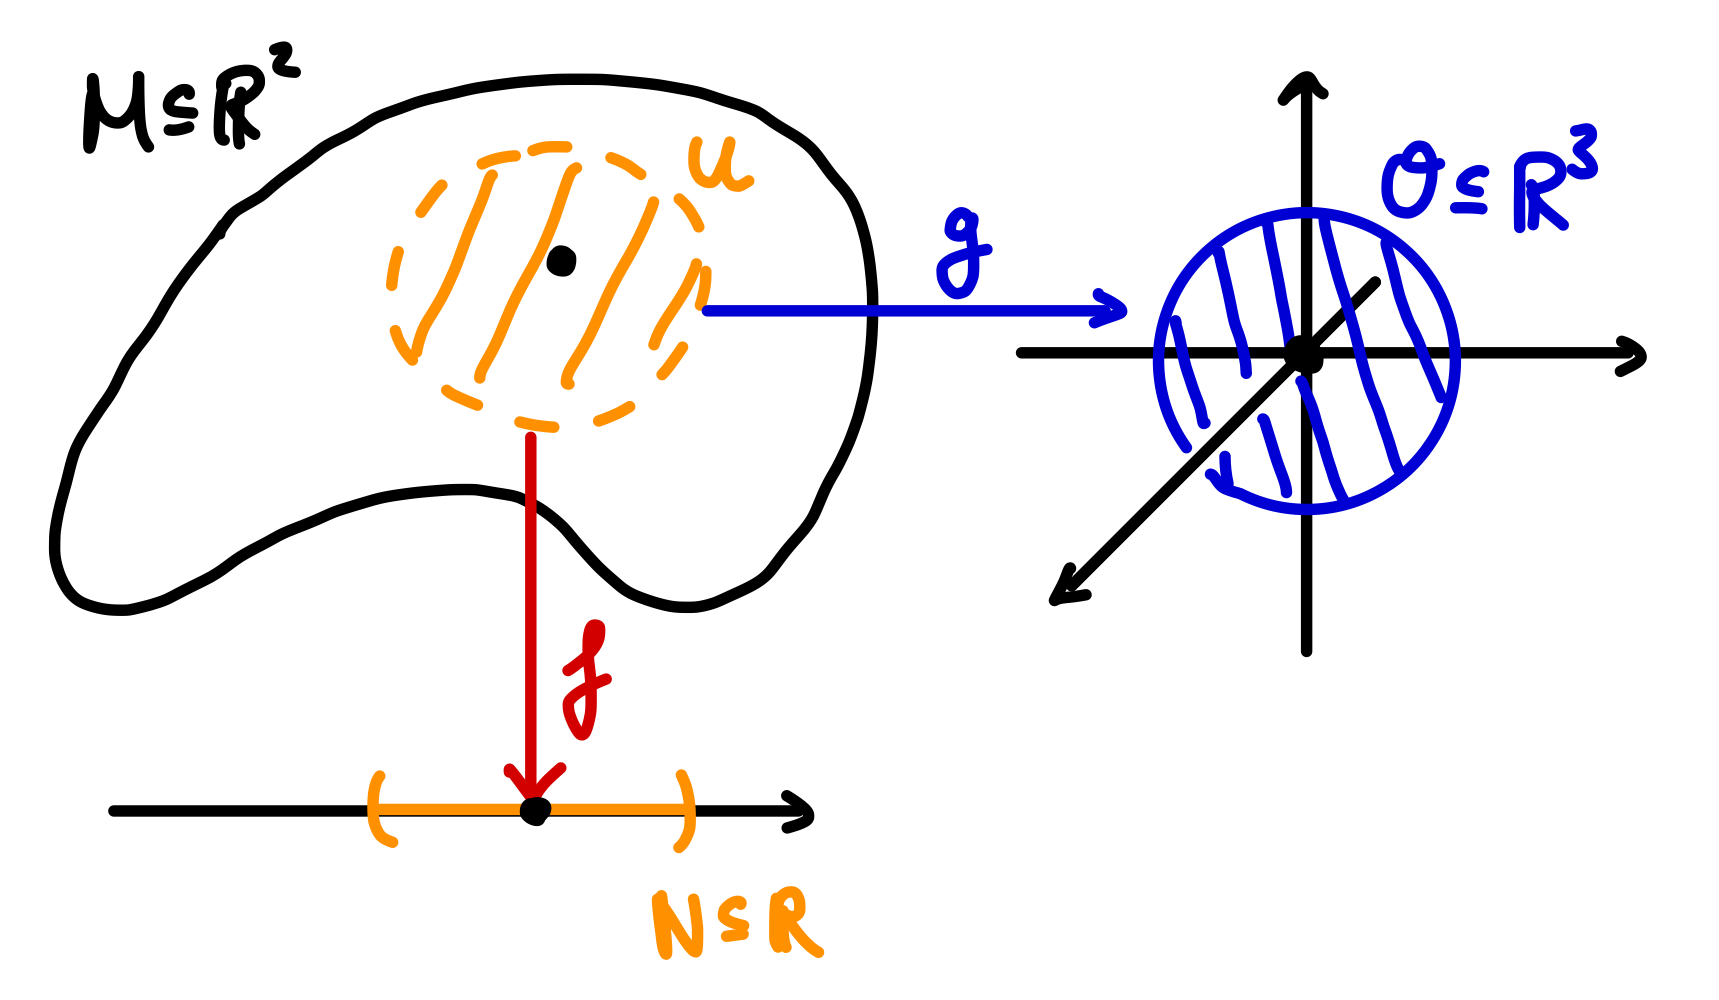
\includegraphics[width=0.3\linewidth]{Bilder/submerimmer.png}
\caption{Lokal sieht eine Submersion $f$ wie eine kanonische Projektion und eine Immersion $g$ wie eine kanonische Injektion aus.}
\end{figure}
\end{satz}
\begin{definition}{Untermannigfaltigkeiten reloaded}{Umfneu}
Seien $N, M$ glatte MFKn. Eine Teilmenge $S \sub M$ heißt \textbf{Untermannigfaltigkeit (UMF)}, falls $S$ das Bild einer Einbettung $f: N \to M$ ist.
\end{definition}
\begin{bemerkung}
Äquivalent ist die Beschreibung von UMF als Teilmengen $U \sub M$ einer MFK $M$, die lokal Urbild eines Punktes unter einer lokal definierten Submersion sind.
\end{bemerkung}
Für $M=\R^n$ erhalten wir wieder unser schon bekanntes Konzept aus \ref{umfn}.
\begin{definition}{Regularität}{reg}
Sei $F: M \to N$ eine glatte Abbildung.\\
Ein Punkt $p \in M$ heißt \textbf{regulär für} $F$, falls $F_{\ast, p}: T_pM \to T_{F(p)}N$ surjektiv ist. Andernfalls heißt $p$ \textbf{kritisch} für $F$.\\
Ein Punkt $q \in N$ heißt \textbf{regulärer Wert von} $F$, falls $F^{-1}(q)$ nur aus regulären Punkten besteht. Wenn $F^{-1}(q)$ mindestens einen kritischen Punkt enthält, heißt $q \in N$ \textbf{kritischer Wert}.
\end{definition}
\begin{figure}[H]
\label{fig:kritisch}
\centering
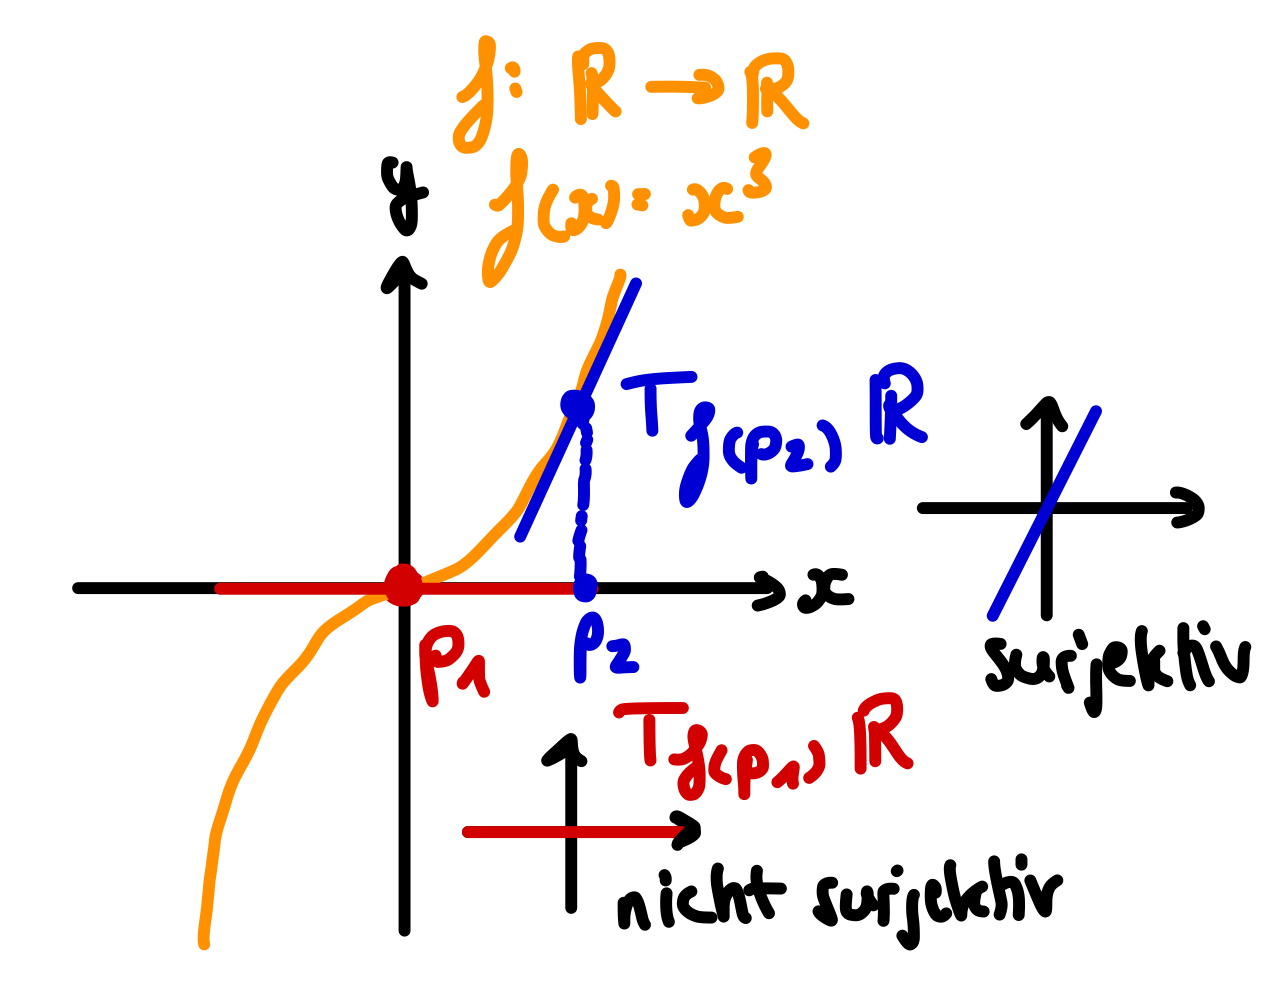
\includegraphics[width=0.3\linewidth]{Bilder/bspkritisch.png}
\caption{Für die Funktion $f: \R \to \R, \ x \mapsto x^3$ ist $p=0$ kritisch.}
\end{figure}
\begin{satz}{Satz vom regulären Wert}{regwertsatz}
Sei $F: M \to N$ eine glatte Abbildung und $q \in N$ ein regulärer Wert von $F$.\\
Dann ist $F^{-1}(q) \sub M$ eine glatte UMF von $M$ der Dimension $\dim M - \dim N$. Für $p \in F^{-1}(q)$ gilt außerdem $T_pF^{-1} (q) = \ker F_{\ast, p}$.
\begin{figure}[H]
\label{fig:regulaer}
\centering
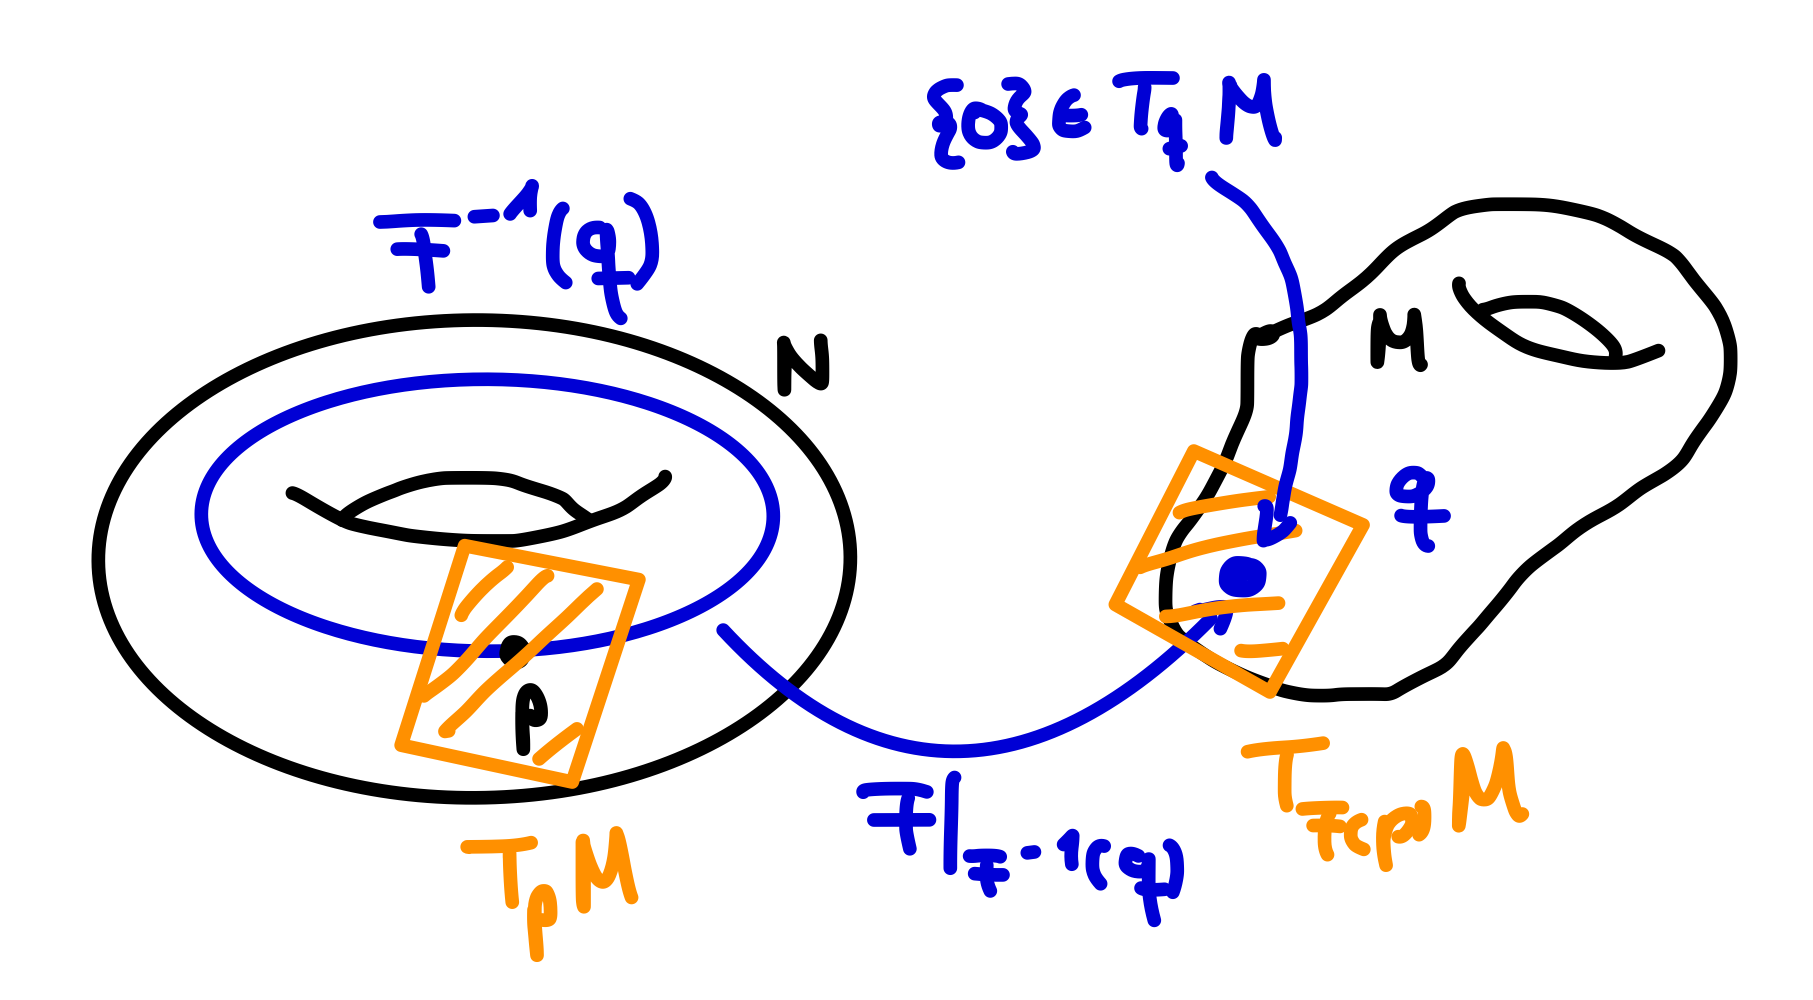
\includegraphics[width=0.3\linewidth]{Bilder/regulaer.png}
\caption{Das Urbild von $q$ unter $F$ sind die Niveaulinien von $F$, die eine UMF von $M$ darstellen.}
\end{figure}
\end{satz}
\begin{bemerkung}
Für $M = \R^n$ und $N= \R^k$ erhalten wir eine unserer äquivalenten Charakterisierungen von UMFn. Der allgemeine Fall folgt aus dem Spezialfall, indem man mit lokalen Karten arbeitet. Die Nützlichkeit des Satzes ergibt sich aus folgendem Satz.
\end{bemerkung}
\begin{satz}{Satz von Sard}{sard}
Sei $F: M \to N$ eine glatte Abbildung.\\
Dann hat die Menge der kritischen Werte von $F$ Lebesgue-Maß $0$ in $N$, die Menge der regulären Werte ist also dicht.
\end{satz}
\begin{bemerkung}
$A \sub N$ hat Lebesgue-Maß $0$, falls für jede Karte $\phi: U \to V \sub \R^k$ die Menge $\phi(A \cap U) \sub \R^k$ Lebesgue-Maß $0$ hat.
\end{bemerkung}
\begin{definition}{\textit{Transversalität}}{transvers}
Seien $M,N$ glatte MFKn und $F: M \to N$ glatt. Sei $S \sub N$ eine UMF. $F$ heißt \textbf{transvers} zu $S$, falls in allen $p \in M$ mit $F(p) \in S$ gilt:
\begin{equation}
F_{\ast, p} (T_pM) + T_{F(p)}S=T_{F(p)}N.
\end{equation}
\end{definition}
\begin{satz}{\textit{UMF als Urbilder transverser Abbildungen}}{transversumf}
Ist $F$ transvers zu $S$, so ist $F^{-1} \sub M$ eine UMF mit Dimension
\begin{equation}
\dim F^{-1} = \dim M + \dim S - \dim N.
\end{equation}
\end{satz}
\begin{beweis}
Übung (A8)
\end{beweis}
\begin{satz}{\textit{Einbettungen als injektive Immersionen}}{injektiveinbettung}
Seien $M,N$ glatte MFKn und sei $M$ darüber hinaus kompakt. Sei weiterhin $F: M \to N$ eine \textcolor{red}{injektive Immersion}. Dann ist $F$ eine Einbettung.\\
Gilt $\dim M = \dim N$ und ist $N$ zusammenhängend, so ist $F$ ein Diffeomorphismus.
\end{satz}
\begin{beweis}
Übung (A10)
\end{beweis}
